\chapter{Creatures}
\label{ch:creatures}

In Fantasy D100, monsters can be as richly detailed as the characters themselves. As well as characteristics they have skills, weapons and supernatural abilities. They are not mere cannon fodder to be killed and looted. They have their own motives that often bring them into conflict with the player characters, and if sentient can be used to create player characters.

This chapter contains several creatures grouped in lists according to their special characteristics; animals, spirits, undead, etc. It is encouraged (if not strongly recommended) that Game Masters create campaign-specific monsters using this section's material as examples.
\vspace{1em}

\begin{rpg-titlebox}{Monsters as Player Characters}
Although in theory many of the monsters in this chapter can be used as player characters the following are especially suited: Dwarf, Elf, Centaur, Goblin, Orc, Ogre, Lizardman.
\end{rpg-titlebox}
  
The following characteristics, attributes, skills, and special rules, collectively known as a ‘Stat block’, for each of the creatures listed on the Monsters List, are the bare bones of a creature. You can use them straight away to give an average non-descript member of that race.

To create creatures that truly fit the adage “Monsters are People too”, take the Stat block and use it as a base for a complete character. Think of a concept for the character and then add the skills, characteristics and supernatural abilities that the character needs. You may want to generate the creature character as if it was a player character. This often creates good opposition for the players, since the creature will be of comparable experience. 

Note that you should be careful with increasing encounter difficulty by increasing numbers of monsters. A much better way is to increase the power of individual monsters, by increasing skills and supernatural abilities, to be closer to the player character power level.  Fantasy D100 combat works best when there is roughly the same amount of monsters as player characters.

\begin{figure}
\begin{center}
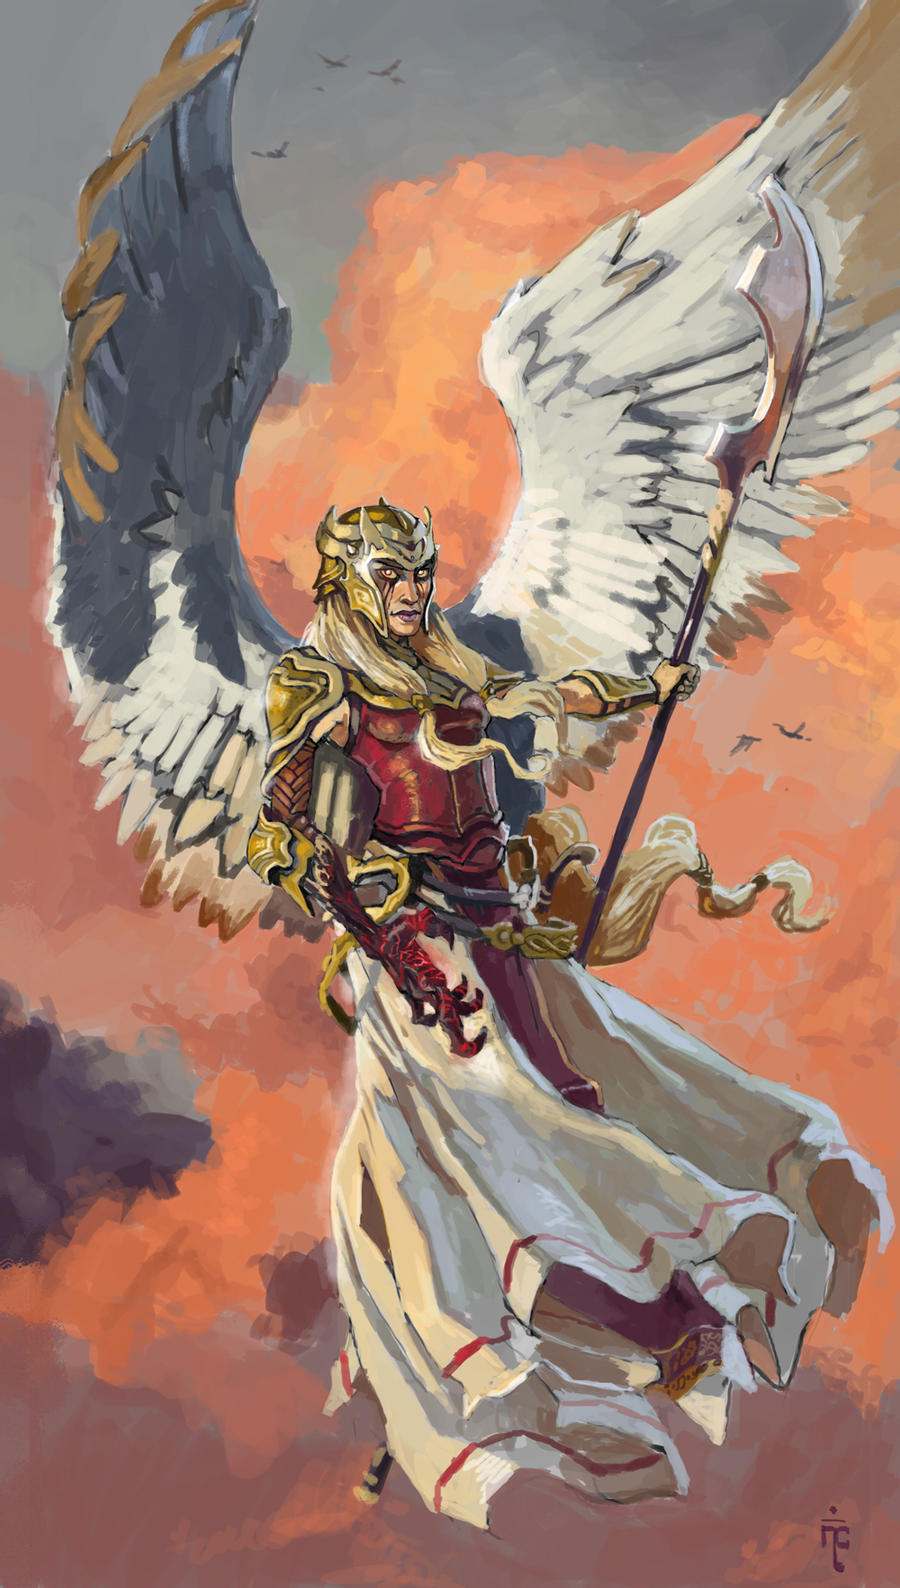
\includegraphics[scale=0.27]{img/corruption_by_ncorva.jpg}
\end{center}
\end{figure}


\clearpage

\section{Animals}

This list describes more mundane animals. It lists domestic animals (such as horses and dogs), as well as wild beasts. Some of the animals are in their ‘Giant’ form, which are more threatening opponents than their normal species.

None of the animals listed here have any treasure by design. They may have some as determined by the Gamemaster as fits the needs of the story. For example a carnivore may have a few trinkets In the remains of its previous meals.

All the Animals listed here are of fixed INT and therefore not sentient. They have a Dodge, Persistence and Resilience of DEX x3, Pow x3, CON x3 respectively and none of them know have any supernatural abilities.

\vspace{1em}

\begin{samepage}
\begin{monsterbox}{Ant (Giant)}
	\basics[%
        hitpoints  = 12, 
	majorwound = 6,
	damagemodifier = 0,
	powerpoints = 6,
	movementrate = 15m,
	armor = Chitin (5 AP),
	]
	\rpghline%
	\stats[ % This stat command will autocomplete the modifier for you
		STR = 4D6   (14),
		CON = 3D6+6 (17),
		DEX = 2D6+6 (13),
		SIZ = 2D6   (7),
		INT = 2     (2),
		POW = 1D6+3 (6),
		CHA = 5     (5)
	]
	%\rpghline%
	%\details[%
	% If you want to use commas in these sections, enclose the
	% description in braces.
	% I'm so sorry.
	%languages = {Common Lisp, Erlang},
	%]
	\rpghline%
	\rpgmonstersection{Skills}
	\begin{rpg-monsteraction}[Unarmed Combat 50\%]
		Bite (1D6)
	\end{rpg-monsteraction}
\end{monsterbox}
\end{samepage}


\begin{samepage}
\begin{monsterbox}{Bear}
	\basics[%
        hitpoints  = 19, 
	majorwound = 10,
	damagemodifier = 0,
	powerpoints = 11,
	movementrate = 23m,
	armor = Tough hide (3 AP),
	]
	\rpghline%
	\stats[ % This stat command will autocomplete the modifier for you
		STR = 3D6+15 (25),
		CON = 2D6+6  (13),
		DEX = 3D6    (11),
		SIZ = 3D6+15 (25),
		INT = 5     (5),
		POW = 3D6   (11),
		CHA = 5     (5)
	]
	%\rpghline%
	%\details[%
	% If you want to use commas in these sections, enclose the
	% description in braces.
	% I'm so sorry.
	%languages = {Common Lisp, Erlang},
	%]
	\rpghline%
	\rpgmonstersection{Skills}
	\begin{rpg-monsteraction}[Unarmed Combat 60\%]
		Bite (1D8+2D6), Claw (1D6+2D6)
	\end{rpg-monsteraction}
\end{monsterbox}
\end{samepage}

\begin{samepage}
\begin{monsterbox}{Bull}
	\basics[%
        hitpoints  = 15, 
	majorwound = 8,
	damagemodifier = +1D6,
	powerpoints = 7,
	movementrate = 15m,
	armor = Hide (2 AP),
	]
	\rpghline%
	\stats[ % This stat command will autocomplete the modifier for you
		STR = 4D6+6 (20),
		CON = 2D6+9 (15),
		DEX = 2D6   (7),
		SIZ = 2D6+9 (15),
		INT = 4     (4),
		POW = 2D6   (7),
		CHA = 4     (4)
	]
	%\rpghline%
	%\details[%
	% If you want to use commas in these sections, enclose the
	% description in braces.
	% I'm so sorry.
	%languages = {Common Lisp, Erlang},
	%]
	\rpghline%
	\rpgmonstersection{Skills}
	\begin{rpg-monsteraction}[Unarmed Combat 40\%]
		Charge (1D8+1D6), Trample (1D8+1D6)
	\end{rpg-monsteraction}
\end{monsterbox}
\end{samepage}


\begin{samepage}
\begin{monsterbox}{Crocodile}
	\basics[%
        hitpoints  = 15, 
	majorwound = 8,
	damagemodifier = +1D6,
	powerpoints = 11,
	movementrate = {7m, 2m in water},
	armor = Thich hide (5 AP),
	]
	\rpghline%
	\stats[ % This stat command will autocomplete the modifier for you
		STR = 5D6+12 (30),
		CON = 3D6+12 (19),
		DEX = 3D6    (11),
		SIZ = 4D6    (14),
		INT = 3      (3),
		POW = 3D6    (11),
		CHA = 3      (3)
	]
	%\rpghline%
	%\details[%
	% If you want to use commas in these sections, enclose the
	% description in braces.
	% I'm so sorry.
	%languages = {Common Lisp, Erlang},
	%]
	\rpghline%
	\rpgmonstersection{Skills}
	\begin{rpg-monsteraction}[Unarmed Combat 50\%]
		Bite (1D8+1D6)
	\end{rpg-monsteraction}
\end{monsterbox}
\end{samepage}


\begin{samepage}
\begin{monsterbox}{Dog}
	\basics[%
        hitpoints  = 7, 
	majorwound = 4,
	damagemodifier = 0,
	powerpoints = 9,
	movementrate = 23m,
	armor = None,
	]
	\rpghline%
	\stats[ % This stat command will autocomplete the modifier for you
		STR = 2D6+6 (13),
		CON = 3D6   (11),
		DEX = 2D6+6 (13),
		SIZ = 1D6   (3),
		INT = 5     (5),
		POW = 1D6+6 (9),
		CHA = 5     (5)
	]
	%\rpghline%
	%\details[%
	% If you want to use commas in these sections, enclose the
	% description in braces.
	% I'm so sorry.
	%languages = {Common Lisp, Erlang},
	%]
	\rpghline%
	\rpgmonstersection{Skills}
	\begin{rpg-monsteraction}[Unarmed Combat 40\%]
		Bite (1D6)
	\end{rpg-monsteraction}
\end{monsterbox}
\end{samepage}


\begin{samepage}
\begin{monsterbox}{Elephant}
	\basics[%
        hitpoints  = 36, 
	majorwound = 18,
	damagemodifier = +5D6,
	powerpoints = 13,
	movementrate = 23m,
	armor = Thick hide (3 AP),
	]
	\rpghline%
	\stats[ % This stat command will autocomplete the modifier for you
		STR = 6D6+24 (45),
		CON = 3D6+15 (24),
		DEX = 3D6    (11),
		SIZ = 6D6+30 (48),
		INT = 6      (6),
		POW = 2D6+6  (13),
		CHA = 5      (5)
	]
	%\rpghline%
	%\details[%
	% If you want to use commas in these sections, enclose the
	% description in braces.
	% I'm so sorry.
	%languages = {Common Lisp, Erlang},
	%]
	\rpghline%
	\rpgmonstersection{Skills}
	\begin{rpg-monsteraction}[Unarmed Combat 45\%]
		Trample (1D12+5D6), Tusk (1D10+5D6)
	\end{rpg-monsteraction}
\end{monsterbox}
\end{samepage}

\begin{samepage}
\begin{monsterbox}{Hawk}
	\basics[%
        hitpoints  = 3, 
	majorwound = 2,
	damagemodifier = -1D6,
	powerpoints = 7,
	movementrate = {15m, 30m flying},
	armor = None,
	]
	\rpghline%
	\stats[ % This stat command will autocomplete the modifier for you
		STR = 1D3    (2),
		CON = 2D3    (4),
		DEX = 3D6+18 (27),
		SIZ = 1D2    (2),
		INT = 4      (4),
		POW = 2D6    (7),
		CHA = 4      (4)
	]
	%\rpghline%
	%\details[%
	% If you want to use commas in these sections, enclose the
	% description in braces.
	% I'm so sorry.
	%languages = {Common Lisp, Erlang},
	%]
	\rpghline%
	\rpgmonstersection{Skills}
	\begin{rpg-monsteraction}[Unarmed Combat 50\%]
		Claw (1D6-1D6), Bite (1D4-1D6)
	\end{rpg-monsteraction}
\end{monsterbox}
\end{samepage}


\begin{samepage}
	\begin{monsterbox}{Hawk (Giant)}
	\basics[%
        hitpoints  = 36, 
	majorwound = 18,
	damagemodifier = +4D6,
	powerpoints = 11,
	movementrate = {23m, 30m flying},
	armor = Thick feathers (3 AP),
	]
	\rpghline%
	\stats[ % This stat command will autocomplete the modifier for you
		STR = 6D6+21 (39),
		CON = 5D6+15 (33),
		DEX = 3D6+9  (18),
		SIZ = 6D6+21 (39),
		INT = 4      (4),
		POW = 3D6    (11),
		CHA = 4      (4)
	]
	%\rpghline%
	%\details[%
	% If you want to use commas in these sections, enclose the
	% description in braces.
	% I'm so sorry.
	%languages = {Common Lisp, Erlang},
	%]
	\rpghline%
	\rpgmonstersection{Skills}
	\begin{rpg-monsteraction}[Unarmed Combat 80\%]
		Claw (1D8+4D6), Bite (1D6+4D6)
	\end{rpg-monsteraction}
\end{monsterbox}
\end{samepage}


\begin{samepage}
\begin{monsterbox}{Horse}
	\basics[%
        hitpoints  = 21, 
	majorwound = 11,
	damagemodifier = +2D6,
	powerpoints = 11,
	movementrate = 30m,
	armor = Hide (2 AP),
	]
	\rpghline%
	\stats[ % This stat command will autocomplete the modifier for you
		STR = 2D6+18 (25),
		CON = 3D6+6  (17),
		DEX = 2D6+3  (10),
		SIZ = 2D6+18 (25),
		INT = 4      (4),
		POW = 3D6    (11),
		CHA = 5      (5)
	]
	%\rpghline%
	%\details[%
	% If you want to use commas in these sections, enclose the
	% description in braces.
	% I'm so sorry.
	%languages = {Common Lisp, Erlang},
	%]
	\rpghline%
	\rpgmonstersection{Skills}
	\begin{rpg-monsteraction}[Unarmed Combat 40\%]
		Kick (1D6+2D6)
	\end{rpg-monsteraction}
\end{monsterbox}
\end{samepage}


\begin{samepage}
\begin{monsterbox}{Lion (Big Cat)}
	\basics[%
        hitpoints  = 15, 
	majorwound = 8,
	damagemodifier = +1D6,
	powerpoints = 11,
	movementrate = 23m,
	armor = Hide (2 AP),
	]
	\rpghline%
	\stats[ % This stat command will autocomplete the modifier for you
		STR = 3D6+12 (24),
		CON = 3D6    (11),
		DEX = 3D6+6  (17),
		SIZ = 2D6+12 (19),
		INT = 5      (5),
		POW = 3D6    (11),
		CHA = 5      (5)
	]
	%\rpghline%
	%\details[%
	% If you want to use commas in these sections, enclose the
	% description in braces.
	% I'm so sorry.
	%languages = {Common Lisp, Erlang},
	%]
	\rpghline%
	\rpgmonstersection{Skills}
	\begin{rpg-monsteraction}[Unarmed Combat 60\%]
		Bite (1D8+1D6), Claw (1D6+1D6)
	\end{rpg-monsteraction}
\end{monsterbox}
\end{samepage}


\begin{samepage}
\begin{monsterbox}{Lizard (Giant)}
	\basics[%
        hitpoints  = 15, 
	majorwound = 8,
	damagemodifier = +1D6,
	powerpoints = 11,
	movementrate = 15m,
	armor = Hide (2 AP),
	]
	\rpghline%
	\stats[ % This stat command will autocomplete the modifier for you
		STR = 2D6+12 (19),
		CON = 3D6    (11),
		DEX = 1D6+12 (15),
		SIZ = 2D6+12 (19),
		INT = 3      (3),
		POW = 3D6    (11),
		CHA = 3      (3)
	]
	%\rpghline%
	%\details[%
	% If you want to use commas in these sections, enclose the
	% description in braces.
	% I'm so sorry.
	%languages = {Common Lisp, Erlang},
	%]
	\rpghline%
	\rpgmonstersection{Skills}
	\begin{rpg-monsteraction}[Unarmed Combat 35\%]
		Bite (1D6+1D6), Tail (1D8+1D6)
	\end{rpg-monsteraction}
\end{monsterbox}
\end{samepage}


\begin{samepage}
\begin{monsterbox}{Octupus (Giant)}
	\basics[%
        hitpoints  = 31, 
	majorwound = 16,
	damagemodifier = +4D6,
	powerpoints = 11,
	movementrate = {7m land, 30m swimming},
	armor = Tough skin (4 AP),
	]
	\rpghline%
	\stats[ % This stat command will autocomplete the modifier for you
		STR = 12D6  (42),
		CON = 4D6+6 (14),
		DEX = 3D6+12 (23),
		SIZ = 12D6   (42),
		INT = 4      (4),
		POW = 3D6    (11),
		CHA = 4      (4)
	]
	%\rpghline%
	%\details[%
	% If you want to use commas in these sections, enclose the
	% description in braces.
	% I'm so sorry.
	%languages = {Common Lisp, Erlang},
	%]
	\rpghline%
	\rpgmonstersection{Skills}
	\begin{rpg-monsteraction}[Unarmed Combat 50\%]
		Bite (1D8+4D6), Arm (1D4+4D6)
	\end{rpg-monsteraction}
\end{monsterbox}
\end{samepage}


\begin{samepage}
\begin{monsterbox}{Python (Giant)}
	\basics[%
        hitpoints  = 11, 
	majorwound = 6,
	damagemodifier = +2D6,
	powerpoints = 11,
	movementrate = 15m,
	armor = Scales (3 AP),
	]
	\rpghline%
	\stats[ % This stat command will autocomplete the modifier for you
		STR = 3D6+24 (35),
		CON = 3D6    (11),
		DEX = 2D6+6  (13),
		SIZ = 3D6    (11),
		INT = 3      (3),
		POW = 3D6    (11),
		CHA = 3      (3)
	]
	%\rpghline%
	%\details[%
	% If you want to use commas in these sections, enclose the
	% description in braces.
	% I'm so sorry.
	%languages = {Common Lisp, Erlang},
	%]
	\rpghline%
	\rpgmonstersection{Skills}
	\begin{rpg-monsteraction}[Unarmed Combat 50\%]
		Bite (1D4+2D6), Constrict (1D8+2D6)
	\end{rpg-monsteraction}
\end{monsterbox}
\end{samepage}


\begin{samepage}
\begin{monsterbox}{Raven}
	\basics[%
        hitpoints  = 3, 
	majorwound = 2,
	damagemodifier = -1D6,
	powerpoints = 7,
	movementrate = {15m, 25m flying},
	armor = None,
	]
	\rpghline%
	\stats[ % This stat command will autocomplete the modifier for you
		STR = 1D3    (2),
		CON = 2D3    (4),
		DEX = 3D6+12 (21),
		SIZ = 1D2    (2),
		INT = 5      (5),
		POW = 2D6    (7),
		CHA = 4      (4)
	]
	%\rpghline%
	%\details[%
	% If you want to use commas in these sections, enclose the
	% description in braces.
	% I'm so sorry.
	%languages = {Common Lisp, Erlang},
	%]
	\rpghline%
	\rpgmonstersection{Skills}
	\begin{rpg-monsteraction}[Unarmed Combat 35\%]
		Claw (1D6-1D6), Bite (1D4-1D6)
	\end{rpg-monsteraction}
\end{monsterbox}
\end{samepage}


\begin{samepage}
\begin{monsterbox}{Rhinoceros}
	\basics[%
        hitpoints  = 19, 
	majorwound = 10,
	damagemodifier = +2D6,
	powerpoints = 11,
	movementrate = 23m,
	armor = Thick hide (5 AP),
	]
	\rpghline%
	\stats[ % This stat command will autocomplete the modifier for you
		STR = 2D6+21 (26),
		CON = 3D6    (11),
		DEX = 2D6    (7),
		SIZ = 2D6+21 (26),
		INT = 3      (3),
		POW = 3D6    (11),
		CHA = 3      (3)
	]
	%\rpghline%
	%\details[%
	% If you want to use commas in these sections, enclose the
	% description in braces.
	% I'm so sorry.
	%languages = {Common Lisp, Erlang},
	%]
	\rpghline%
	\rpgmonstersection{Skills}
	\begin{rpg-monsteraction}[Unarmed Combat 50\%]
		Bite (1D6+2D6), Gore (1D8+2D6), Trample (1D12+2D6)
	\end{rpg-monsteraction}
\end{monsterbox}
\end{samepage}


\begin{samepage}
\begin{monsterbox}{Spider (Giant)}
	\basics[%
        hitpoints  = 22, 
	majorwound = 11,
	damagemodifier = +1D6,
	powerpoints = 11,
	movementrate = {15m on land, 23m in web},
	armor = Chitin (4 AP),
	]
	\rpghline%
	\stats[ % This stat command will autocomplete the modifier for you
		STR = 2D6+12 (19),
		CON = 3D6+6  (17),
		DEX = 2D6+9  (16),
		SIZ = 4D6+12 (26),
		INT = 8      (8),
		POW = 3D6    (11),
		CHA = 2      (2)
	]
	%\rpghline%
	%\details[%
	% If you want to use commas in these sections, enclose the
	% description in braces.
	% I'm so sorry.
	%languages = {Common Lisp, Erlang},
	%]
	\rpghline%
	\rpgmonstersection{Skills}
	\begin{rpg-monsteraction}[Unarmed Combat 50\%]
		Bite (1D6+1D6+Venom), Web
	\end{rpg-monsteraction}
	\rpgmonstersection{Abilities}
	\begin{rpg-monsteraction}[Spider Venom]\\
		\textit{Type:} Ingested or smeared\\
		\textit{Delay:} 1D3 Combat Rounds\\
		\textit{Potency:} Spider's CONx3\\
		\textit{Full Effect:} 1D3 Hit Points per minute and applies –6 penalty to victim’s DEX (upon reaching 0 DEX victim becomes paralysed)\\ 
		\textit{Duration:} 6D10 minutes
	\end{rpg-monsteraction}
	\begin{rpg-monsteraction}[Web]
		Entangles opponent. Success is determined by an opposed check of attack roll vs an Athletics roll. If entangled, the web can be destroyed (POWx2 Hit Points).
	\end{rpg-monsteraction}


\end{monsterbox}
\end{samepage}

\newpage

\begin{samepage}
\begin{monsterbox}{Viper}
	\basics[%
        hitpoints  = 7, 
	majorwound = 4,
	damagemodifier = 0,
	powerpoints = 13,
	movementrate = 30m,
	armor = Scales (1 AP),
	]
	\rpghline%
	\stats[ % This stat command will autocomplete the modifier for you
		STR = 2D6+6  (13),
		CON = 2D6    (6),
		DEX = 3D6+18 (27),
		SIZ = 2D6    (7),
		INT = 3      (3),
		POW = 2D6+6  (13),
		CHA = 3      (3)
	]
	%\rpghline%
	%\details[%
	% If you want to use commas in these sections, enclose the
	% description in braces.
	% I'm so sorry.
	%languages = {Common Lisp, Erlang},
	%]
	\rpghline%
	\rpgmonstersection{Skills}
	\begin{rpg-monsteraction}[Unarmed Combat 60\%]
		Bite (1D6+Venom)
	\end{rpg-monsteraction}
	\rpgmonstersection{Abilities}
	\begin{rpg-monsteraction}[Viper Venom]\\
		\textit{Type:} Ingested or smeared\\
		\textit{Delay:} 1 Combat Round\\
		\textit{Potency:} 48\\
		\textit{Full Effect:} 1D4 Hit Points damage for each minute and -3 CON (upon reaching 0 CON victim dies)\\ 
		\textit{Duration:} 6D10 minutes
	\end{rpg-monsteraction}
\end{monsterbox}
\end{samepage}


\begin{samepage}
\begin{monsterbox}{Wolf}
	\basics[%
        hitpoints  = 12, 
	majorwound = 6,
	damagemodifier = 0,
	powerpoints = 11,
	movementrate = 23m,
	armor = None,
	]
	\rpghline%
	\stats[ % This stat command will autocomplete the modifier for you
		STR = 3D6   (11),
		CON = 3D6+3 (14),
		DEX = 3D6+3 (13),
		SIZ = 2D6+3 (10),
		INT = 5     (5),
		POW = 3D6   (11),
		CHA = 5     (5)
	]
	%\rpghline%
	%\details[%
	% If you want to use commas in these sections, enclose the
	% description in braces.
	% I'm so sorry.
	%languages = {Common Lisp, Erlang},
	%]
	\rpghline%
	\rpgmonstersection{Skills}
	\begin{rpg-monsteraction}[Unarmed Combat 50\%]
		Bite (1D8), Claw (1D6)
	\end{rpg-monsteraction}
\end{monsterbox}
\end{samepage}

\clearpage


%\section{Demons}
%...
%\newpage


\section{Monsters}


\begin{monsterbox}{Basilisk}
	\textit{Born from the egg of a cockerel acted upon in an Alchemist’s or witches cauldron, this magical monster is the product of foul magic. It is a large lizard with multicoloured scales. Its baleful gaze can kill and its blood is poisonous and corrosive.   Basilisks are usually employed as guardians of their master’s treasure.}\\
	\rpghline
	\basics[%
        hitpoints  = 8, %\rpgdice{3d8 + 3},
	majorwound = 4,
	damagemodifier = -1D6,
	powerpoints = 16,
	movementrate = 15m,
	armor = Armor Scales (2AP),
	plunderrating = 5
	]
	\rpghline%
	\stats[ % This stat command will autocomplete the modifier for you
		STR = 2D3   (4),
		CON = 2D6+6 (13),
		DEX = 3D6   (11),
		SIZ = 1D3   (2),
		INT = 3     (3),
		POW = 1D6+12 (16),
		CHA = 3     (3)
	]
	%\rpghline%
	%\details[%
	% If you want to use commas in these sections, enclose the
	% description in braces.
	% I'm so sorry.
	%languages = {Common Lisp, Erlang},
	%]
	\rpghline%
	\rpgmonstersection{Skills}
	\begin{rpg-monsteraction}[Resistances]
		Dodge~40\%, Persistence~50\%, Resilience~70\%
	\end{rpg-monsteraction}
	\begin{rpg-monsteraction}[Knowledge]
    		Natural lore~40\%
	\end{rpg-monsteraction}
	\begin{rpg-monsteraction}[Practical]
		Athletics~65\%, Deception~40\%
	\end{rpg-monsteraction}
	\begin{rpg-monsteraction}[Ranged Combat 100\%]
		Death Gaze (Range: POW in metres)
	\end{rpg-monsteraction}
	\begin{rpg-monsteraction}[Unarmed Combat 35\%]
		Bite (1D6-1D6+poison)
	\end{rpg-monsteraction}
	\rpgmonstersection{Abilities}
	\begin{rpg-monsteraction}[Basilisk Venom \& Poison Blood]\\
		\textit{Type:} Ingested or smeared\\
		\textit{Delay:} Immediate\\
		\textit{Potency:} 65\\
		\textit{Full Effect:} 1D4 Hit Points damage for each minute and -6 CON (upon reaching 0 CON victim dies)\\ 
		\textit{Duration:} 6D10 minutes\\
		Any non-magical weapon hitting the basilisk corrodes in the creature’s blood, completely disintegrating after D4 rounds. The basilisk’s poison and corrosive blood are magical effects, which lose their special properties a few minutes after leaving the basilisk’s body, making it virtually impossible to use the creature as a source for making lethal compounds.
	\end{rpg-monsteraction}
	\begin{rpg-monsteraction}[Death Gaze]
		A basilisk can kill with a glance. In combat the basilisk glares at a single opponent each round. If the basilisk overcomes the target in an opposed test of its Persistence against the target’s Resilience, the target dies instantly. Using the gaze attack costs no Power Points, and the basilisk may attack normally in any round in which it uses the gaze attack. This attack penetrates magical defences as if it were a Magnitude 6 Magic spell. If the target successfully resists the gaze attack, he is unharmed, though he may certainly be targeted again. 
	\end{rpg-monsteraction}

\end{monsterbox}

%\newpage

\begin{monsterbox}{Beastman}
	\textit{Hybrids of animals of beasts and men, they typically take the form of a man with a beast’s head. Tied to the savagery of nature, they react with hostility to man’s attempt to clear the wilderness for cultivation.  }\\
	\rpghline
	\basics[%
        hitpoints  = 16,
	majorwound = 8,
	damagemodifier = +1D4,
	powerpoints = 11,
	movementrate = 15m,
	armor = Leather (2AP),
	plunderrating = 2
	]
	\rpghline%
	\stats[ % This stat command will autocomplete the modifier for you
		STR = 2D6+6  (13),
		CON = 1D6+12 (16),
		DEX = 3D6    (11),
		SIZ = 1D6+12 (16),
		INT = 2D6+6  (13),
		POW = 3D6    (11),
		CHA = 2D6    (7)
	]
	\rpghline%
	\rpgmonstersection{Skills}
	\begin{rpg-monsteraction}[Resistances]
		Dodge~40\%, Persistence~30\%, Resilience~30\%
	\end{rpg-monsteraction}
	\begin{rpg-monsteraction}[Knowledge]
    		Natural lore~70\%
	\end{rpg-monsteraction}
	\begin{rpg-monsteraction}[Practical]
		Deception~40\%
	\end{rpg-monsteraction}
	\begin{rpg-monsteraction}[Close Combat 50\%]
		Club (1D6+1D4), Shortspear (1D6+1D4), Medium Shield (1D6+1D6)
	\end{rpg-monsteraction}
	\begin{rpg-monsteraction}[Unarmed Combat 60\%]
		Head Butt (1D6+1D4)
	\end{rpg-monsteraction}
	\rpgmonstersection{Abilities}
	\begin{rpg-monsteraction}[Supernatural]\\
		Beastmen can usually learn 3 Magnitude points of Magic.
	\end{rpg-monsteraction}

\end{monsterbox}

%\newpage



\begin{monsterbox}{Centaur}
	\textit{Atop of the body of a well-bred and strong horse, this creature has the body of a strong athletic human where the horse’s head should be. The centaur is the raw power and nobility of nature incarnate. Often they act as the self styled protectors of the wilderness, which brings them into conflict with more settled races who encroach on their territory.}\\
	\rpghline
	\basics[%
        hitpoints  = 19, %\rpgdice{3d8 + 3},
	majorwound = 10,
	damagemodifier = +1D6,
	powerpoints = 11,
	movementrate = 23m,
	armor = Leather (2AP),
	plunderrating = 2
	]
	\rpghline%
	\stats[ % This stat command will autocomplete the modifier for you
		STR = 3D6+6 (17),
		CON = 3D6   (11),
		DEX = 3D6+3 (14),
		SIZ = 4D6+12 (26),
		INT = 2D6+6 (13),
		POW = 3D6   (11),
		CHA = 3D6   (11)
	]
	%\rpghline%
	%\details[%
	% If you want to use commas in these sections, enclose the
	% description in braces.
	% I'm so sorry.
	%languages = {Common Lisp, Erlang},
	%]
	\rpghline%
	\rpgmonstersection{Skills}
	\begin{rpg-monsteraction}[Resistances]
		Dodge~30\%, Persistence~45\%, Resilience~60\%
	\end{rpg-monsteraction}
	\begin{rpg-monsteraction}[Knowledge]
    		Natural lore~60\%
	\end{rpg-monsteraction}
	\begin{rpg-monsteraction}[Practical]
		Athletics~60\%, Performance~50\%, Perception~40\%, Deception~30\%
	\end{rpg-monsteraction}
	\begin{rpg-monsteraction}[Ranged Combat 70\%]
		Longbow (1D10+1D6)
	\end{rpg-monsteraction}
	\begin{rpg-monsteraction}[Close Combat 40\%]
		Lance (1D10+1D6), Medium Shield (1D6+1D6), Arming Sword (1D8+1D6)
	\end{rpg-monsteraction}
	\begin{rpg-monsteraction}[Unarmed Combat 40\%]
		Kick (1D6+1D6)
	\end{rpg-monsteraction}
	\rpgmonstersection{Abilities}
	\begin{rpg-monsteraction}[Supernatural]
		Typically supernatural abilities that are related to Battle, Earth and Nature are available to Centaurs.
	\end{rpg-monsteraction}
	\begin{rpg-monsteraction}[Exceptional Archers]
		Centaurs can use their damage modifier when using bows.
	\end{rpg-monsteraction}

\end{monsterbox}

%\newpage


\begin{monsterbox}{Dragon}
	\textit{These giant flying reptilian monsters are incredibly powerful and dangerous. Dragons are very individual in their temperament. Some are evil cruel beasts. Others are solitary hoarding creatures. Some use their high intelligence to lord it over lesser races.}\\
	\rpghline
	\basics[%
        hitpoints  = 50, %\rpgdice{3d8 + 3},
	majorwound = 25,
	damagemodifier = +7D6,
	powerpoints = 26,
	movementrate = {30m, 45m when flying},
	armor = Dragon Scales (12AP),
	plunderrating = 5-6
	]
	\rpghline%
	\stats[ % This stat command will autocomplete the modifier for you
		STR = 20D6    (70),
		CON = 10D6    (35),
		DEX = 4D6     (14),
		SIZ = 10D6+30 (65),
		INT = 6D6     (21),
		POW = 4D6+12  (26),
		CHA = 6D6     (21)
	]
	%\rpghline%
	%\details[%
	% If you want to use commas in these sections, enclose the
	% description in braces.
	% I'm so sorry.
	%languages = {Common Lisp, Erlang},
	%]
	\rpghline%
	\rpgmonstersection{Skills}
	\begin{rpg-monsteraction}[Resistances]
		Dodge~30\%, Persistence~180\%, Resilience~120\%
	\end{rpg-monsteraction}
	\begin{rpg-monsteraction}[Knowledge]
		Natural lore~100\%, Culture (local) 100\%
	\end{rpg-monsteraction}
	\begin{rpg-monsteraction}[Practical]
		Athletics~120\%, Influence~150\%, Perception~110\%
	\end{rpg-monsteraction}
	\begin{rpg-monsteraction}[Unarmed Combat 125\%]
		Bite (1D10+7D6), Claw (1D8+7D6), Tail (1D20+7D6)
	\end{rpg-monsteraction}
	\rpgmonstersection{Abilities}
	\begin{rpg-monsteraction}[Double Claw Attack]
		In a single Combat Round a dragon can make two claw attacks.
	\end{rpg-monsteraction}
	\begin{rpg-monsteraction}[Breathe Flame]
		The Dragon may breathe flame over an area as a Combat Action. The flame will cover a cone in front of the Dragon, which stretches for its POW in metres. At its furthest extent, the cone is equal to the creature’s POW in width.
		Any creature caught in the flame suffers 4D6 fire damage, though on a successful Dodge roll a character may dive for cover to halve this damage and AP counts as normal.
		The Dragon may only breathe flame once per hour. Further attempts to breathe flame within this time period require the creature to make a Resilience test, with a cumulative –20\% penalty for every attempt.
	\end{rpg-monsteraction}
	\begin{rpg-monsteraction}[Supernatural]
		Dragons are highly magical creatures and often learn Arcane Magic and Magic (of which they have a minimum of 10 points of Magnitude of spells)
	\end{rpg-monsteraction}
\end{monsterbox}

%\newpage


\label{creature:dwarf}
\begin{monsterbox}{Dwarf}
	\textit{These short, stocky and bearded, human-like creatures, live underground in vast halls, meticulously carved out of the rock by their highly skilled hands.  Long lived and proud of their work, Dwarfs are the natural enemies of Orcs and Goblins, who often encroach upon their realms.}\\
	\rpghline
	\basics[%
        hitpoints  = 15, %\rpgdice{3d8 + 3},
	majorwound = 8,
	damagemodifier = 0,
	powerpoints = 11,
	movementrate = 12m,
	armor = Chainmail (5AP),
	plunderrating = 3
	]
	\rpghline%
	\stats[ % This stat command will autocomplete the modifier for you
		STR = 4D6   (14),
		CON = 2D6+12 (19),
		DEX = 3D6   (11),
		SIZ = 1D6+3 (7),
		INT = 2D6+6 (13),
		POW = 3D6   (11),
		CHA = 3D6   (11)
	]
	%\rpghline%
	%\details[%
	% If you want to use commas in these sections, enclose the
	% description in braces.
	% I'm so sorry.
	%languages = {Common Lisp, Erlang},
	%]
	\rpghline%
	\rpgmonstersection{Skills}
	\begin{rpg-monsteraction}[Resistances]
		Dodge~20\%, Persistence~40\%, Resilience~55\%
	\end{rpg-monsteraction}
	\begin{rpg-monsteraction}[Knowledge]
    		Craft~70\%
	\end{rpg-monsteraction}
	\begin{rpg-monsteraction}[Practical]
		Athletics~50\%, Engineering~35\%, Trade~60\%, Mechanisms~40\%
	\end{rpg-monsteraction}
	\begin{rpg-monsteraction}[Close Combat 65\%]
		War Hammer (1D8), Battleaxe (1D8), Medium Shield (1D6)
	\end{rpg-monsteraction}
	\begin{rpg-monsteraction}[Ranged Combat 45\%]
		Light Crossbow (1D8)
	\end{rpg-monsteraction}
	\rpgmonstersection{Abilities}
	\begin{rpg-monsteraction}[Supernatural]
		Typically supernatural abilities that are related to Battle, Earth and Metals are available to Dwarves.
	\end{rpg-monsteraction}
	\begin{rpg-monsteraction}[Thermoception]
		Dwarves can see at dark as if it was day, by detecting heat and cold.
	\end{rpg-monsteraction}
	\begin{rpg-monsteraction}[Earth Sense]
		Dwarfs can automatically sense how far they are underground and whether or not the tunnels or chambers they are in are structurally sound.
	\end{rpg-monsteraction}

\end{monsterbox}

%\newpage

\begin{monsterbox}{Elemental}
\label{monster:elemental}
	\textit{These are magical beings of raw elemental power that come from the Other Worlds. They are usually called or summoned to the mundane world to do the bidding of Priests and Arcane Magic users. Their appearance can vary. Some representative elementals can be seen below.}\\
	\rpghline
	\rpgmonstersection{Types}
	\begin{rpg-monsteraction}[Undines]
		Water elementals that look like a featureless humanoid made of water whose legs dissolve into a pillar then pool of water.\\
		\textit{Type of attack:} Drown\\
		\textit{Resistance used:} Resilience\\
		\textit{Attribute damage:} Hit Points
	\end{rpg-monsteraction}
	\begin{rpg-monsteraction}[Shades]
    		Darkness elementals that are living blobs of darkness.\\
		\textit{Type of attack:} Fear\\
		\textit{Resistance used:} Persistence\\
		\textit{Attribute damage:} Power Points\\
		Shades attack using Fear, when they reduce their opponent’s Power Point’s total to zero they literally die of shock.
	\end{rpg-monsteraction}
	\begin{rpg-monsteraction}[Salamanders]
		Fire elementals that look like lizards made of fire.\\
		\textit{Type of attack:} Burning\\
		\textit{Resistance used:} Resilience\\
		\textit{Attribute damage:} Hit Points
	\end{rpg-monsteraction}
	\begin{rpg-monsteraction}[Gnomes]
		Earth elementals that look like humanoids made of rock.\\
		\textit{Type of attack:} Crush\\
		\textit{Resistance used:} Resilience\\
		\textit{Attribute damage:} Hit Points
	\end{rpg-monsteraction}
	\begin{rpg-monsteraction}[Sylphs]
		Air elementals that take the form of clouds which fly.\\
		\textit{Type of attack:} Buffet\\
		\textit{Resistance used:} Resilience\\
		\textit{Attribute damage:} Hit Points
	\end{rpg-monsteraction}
	\rpgmonstersection{Abilities}
	\begin{rpg-monsteraction}[Attributes]
		The only Stat that an elemental has is SIZ, all its derived attributes and skills are based on this (see table~\ref{tab:elemental-attributes-skills}). Elementals attack by engulfing their enemies. All opponents within the area of attack are potential targets. Elementals use their Attack percentage, which is equal to their size times five, to hit the target who then resists using the resistance appropriate to the attack.
	\end{rpg-monsteraction}
	\begin{rpg-monsteraction}[Immunities]
		Diseases and Poisons
	\end{rpg-monsteraction}
	\begin{rpg-monsteraction}[See Invisible]
		Elementals have magical senses that allow them to ‘see’ invisible creatures, such as immaterial spirits. They also gain a +40\% when detecting hidden characters.
	\end{rpg-monsteraction}
	\begin{rpg-monsteraction}[Camouflage]
		All elementals have the equivalent of a 80\% Deception when lying next to a environment of the same element as themselves. For example, undines are nearly invisible when lying in a pool of water and Gnomes can curl up and blend into a surrounding rocky area.
	\end{rpg-monsteraction}

\end{monsterbox}

\begin{table*}
\begin{center}
\caption{Elemental Attributes and Skills}
\label{tab:elemental-attributes-skills}
\begin{rpg-table}[|l|c|c|Y|Y|Y|Y|c|c|c|]
	\hline
	\textbf{Size}  & \textbf{SIZ} & \textbf{Damage} & \textbf{Hit Points (=SIZ)} & \textbf{Attack (=SIZx5)} & \textbf{Area of attack (=SIZ/5)} & \textbf{Movement rate} & \textbf{Dodge} & \textbf{Persistence} & \textbf{Resilience}\\
	\hline
	Small     & 3  & 1D6 & 3  & 15\%  & 1m  & 15m & 120 & 30  & 100\\
	Medium    & 9  & 2D6 & 9  & 45\%  & 3m  & 23m & 90  & 60  & 100\\
	Large     & 21 & 3D6 & 21 & 105\% & 7m  & 30m & 60  & 90  & 100\\
	Small     & 50 & 4D6 & 50 & 250\% & 16m & 45m & 30  & 120 & 100\\
	\hline
\end{rpg-table}
\end{center}
\end{table*}


%\newpage

\label{creature:elf}
\begin{monsterbox}{Elf}
	\textit{Forest dwellers, these creatures are slender and tall, with ears that end in a point. Haughty and proud, they do not suffer the ravages of time like other mortal races. Tightly bound to their forest realms in ways no human can understand, they often come into conflict with those who despoil their lands.}\\
	\rpghline
	\basics[%
        hitpoints  = 11, 
	majorwound = 6,
	damagemodifier = 0,
	powerpoints = 13,
	movementrate = 15m,
	armor = Leather (2AP),
	plunderrating = 1
	]
	\rpghline%
	\stats[ % This stat command will autocomplete the modifier for you
		STR = 2D6+3 (10),
		CON = 3D6   (11),
		DEX = 3D6+6 (17),
		SIZ = 2D6+3 (10),
		INT = 3D6+6 (17),
		POW = 2D6+6 (13),
		CHA = 3D6   (11)
	]
	%\rpghline%
	%\details[%
	% If you want to use commas in these sections, enclose the
	% description in braces.
	% I'm so sorry.
	%languages = {Common Lisp, Erlang},
	%]
	\rpghline%
	\rpgmonstersection{Skills}
	\begin{rpg-monsteraction}[Resistances]
		Dodge~55\%, Persistence~55\%, Resilience~20\%
	\end{rpg-monsteraction}
	\begin{rpg-monsteraction}[Knowledge]
    		Nature lore~80\%
	\end{rpg-monsteraction}
	\begin{rpg-monsteraction}[Practical]
		Athletics~55\%, Deception~55\%, Perception~30\%, Healing~50\%
	\end{rpg-monsteraction}
	\begin{rpg-monsteraction}[Close Combat 60\%]
		Longspear (1D8)
	\end{rpg-monsteraction}
	\begin{rpg-monsteraction}[Ranged Combat 80\%]
		Shortbow (1D8)
	\end{rpg-monsteraction}
	\rpgmonstersection{Abilities}
	\begin{rpg-monsteraction}[Supernatural]
		Typically supernatural abilities that are related to Battle, Healing and Nature are available to Elves.
	\end{rpg-monsteraction}
	\begin{rpg-monsteraction}[Night Sight]
		Elves treat partial darkness as illuminated and darkness as only partial darkness.
	\end{rpg-monsteraction}
	\begin{rpg-monsteraction}[Exceptional Archers]
		Elves can use their damage modifier when using bows.
	\end{rpg-monsteraction}

\end{monsterbox}

%\newpage

\begin{monsterbox}{Gargoyle}
	\textit{Grotesque humanoids with leathery bat-like wings, their faces with exaggerated features, and large fangs that protrude from their lower jaws. Their skin is a dull grey, meaning that they are often mistaken for statues, a fact that a predatory Gargoyle will often use to its advantage, staying still for hours upon end, until prey comes near. It is rumoured that once the Gargoyles had a vast underground Empire, but now they are encountered in small groups of twenty at the most. Often they find themselves drafted into Orc war bands as flying troops.}\\
	\rpghline
	\basics[%
        hitpoints  = 14,
	majorwound = 7,
	damagemodifier = +2D6,
	powerpoints = 11,
	movementrate = {15m, 23m flying},
	armor = Tough Hide (6AP),
	plunderrating = 0
	]
	\rpghline%
	\stats[ % This stat command will autocomplete the modifier for you
		STR = 5D6+12 (29),
		CON = 3D6    (11),
		DEX = 3D6    (11),
		SIZ = 5D6    (17),
		INT = 1D6    (4),
		POW = 3D6    (11),
		CHA = 1D6    (4)
	]
	\rpghline%
	\rpgmonstersection{Skills}
	\begin{rpg-monsteraction}[Resistances]
		Dodge~25\%, Persistence~40\%, Resilience~40\%
	\end{rpg-monsteraction}
	\begin{rpg-monsteraction}[Knowledge]
    		Natural lore~40\%
	\end{rpg-monsteraction}
	\begin{rpg-monsteraction}[Practical]
		Athletics~40\%, Deception~30\%, Perception~40\%
	\end{rpg-monsteraction}
	\begin{rpg-monsteraction}[Unarmed Combat 50\%]
		Claw (1D6+2D6)
	\end{rpg-monsteraction}
	\rpgmonstersection{Abilities}
	\begin{rpg-monsteraction}[Supernatural]
		Gargolyes tend not to learn magic unless taught it. If some one is stupid enough to teach them magic, it is usually very low Magnitude Magic (max 3), enough to make them useful as troops, but not enough to give them the upper hand in any mutiny.
	\end{rpg-monsteraction}

\end{monsterbox}

%\newpage



\begin{monsterbox}{Giant}
	\textit{Standing at least six metres high, a Giant is a marvel to behold to the ‘little’ races that it towers over. It is rumoured that they once had their own civilisation, one that challenged that of the Gods, and so they were cast down and scattered. Giants are human-like and tend to take on the cultural aspects of the nearest human culture, which they often trade with. That said, many are primitive barbarians in the wilderness. living outside and beyond human society. Some are master stone masons so are found in the mountains where there is an abundance of stone. }\\
	\rpghline
	\basics[%
        hitpoints  = 44,
	majorwound = 22,
	damagemodifier = +5D6,
	powerpoints = 11,
	movementrate = 30m,
	armor = Tough Hide (3AP),
	plunderrating = 1-5
	]
	\rpghline%
	\stats[ % This stat command will autocomplete the modifier for you
		STR = 9D6+18 (49),
		CON = 6D6+18 (39),
		DEX = 2D6+3  (10),
		SIZ = 9D6+18 (49),
		INT = 3D6    (11),
		POW = 3D6    (11),
		CHA = 2D6    (7)
	]
	\rpghline%
	\rpgmonstersection{Skills}
	\begin{rpg-monsteraction}[Resistances]
		Dodge~10\%, Persistence~25\%, Resilience~80\%
	\end{rpg-monsteraction}
	\begin{rpg-monsteraction}[Knowledge]
    		Natural lore~20\%
	\end{rpg-monsteraction}
	\begin{rpg-monsteraction}[Practical]
		Athletics~50\%, Perception~40\%, Deception~5\%
	\end{rpg-monsteraction}
	\begin{rpg-monsteraction}[Close Combat 90\%]
		Huge Club (2D6+5D6)
	\end{rpg-monsteraction}
	\begin{rpg-monsteraction}[Ranged Combat 35\%]
		Thrown boulder (2D6+5D6)
	\end{rpg-monsteraction}
	\begin{rpg-monsteraction}[Unarmed Combat 75\%]
		Stomp (1D6+5D6)
	\end{rpg-monsteraction}
	\rpgmonstersection{Abilities}
	\begin{rpg-monsteraction}[Supernatural]
		Giants tend to learn the magic of those cultures nearest them. Giants who are isolated in the mountains learn Magic, with more powerful individuals becoming Shamans.
	\end{rpg-monsteraction}
	\begin{rpg-monsteraction}[Other Giant Sizes]
		The above Characteristics are for a giant that stands six metres tall. For every additional two metres of height, a giant rolls an additional of 3D6+6 for STR, 2D6+6 for CON and 3D6+6 for SIZ.
	\end{rpg-monsteraction}
\end{monsterbox}

%\newpage



\begin{monsterbox}{Goblin}
	\textit{Sneakier crueller cousins of the Orcs, goblins are a quarrelsome bunch of green-skinned humanoids. They stand as tall as a human child and their smiling faces are dominated by large hooked noses and mouth full of razor-sharp teeth. Constantly in the shadow of the larger humanoid races, often used as slaves or cannon fodder, these diminutive psychopaths take out their frustration on any other creatures unlucky enough to be outnumbered by them or in their power.}\\
	\rpghline
	\basics[%
        hitpoints  = 9, %\rpgdice{3d8 + 3},
	majorwound = 5,
	damagemodifier = 0,
	powerpoints = 10,
	movementrate = 15m,
	armor = Leather (2AP),
	plunderrating = 1
	]
	\rpghline%
	\stats[ % This stat command will autocomplete the modifier for you
		STR = 2D6+3 (10),
		CON = 2D6+3 (10),
		DEX = 5D6   (17),
		SIZ = 2D6   (7),
		INT = 3D6   (11),
		POW = 2D6+3 (10),
		CHA = 2D6   (7)
	]
	%\rpghline%
	%\details[%
	% If you want to use commas in these sections, enclose the
	% description in braces.
	% I'm so sorry.
	%languages = {Common Lisp, Erlang},
	%]
	\rpghline%
	\rpgmonstersection{Skills}
	\begin{rpg-monsteraction}[Resistances]
		Dodge~50\%, Persistence~20\%, Resilience~35\%
	\end{rpg-monsteraction}
	\begin{rpg-monsteraction}[Knowledge]
    		Natural lore~50\%
	\end{rpg-monsteraction}
	\begin{rpg-monsteraction}[Practical]
		Athletics~50\%, Perception~35\%, Deception~75\%, Mechanisms~50\%
	\end{rpg-monsteraction}
	\begin{rpg-monsteraction}[Close Combat 40\%]
		Shortspear (1D6), Small Shield (1D4)
	\end{rpg-monsteraction}
	\begin{rpg-monsteraction}[Ranged Combat 50\%]
		Sling (1D6)
	\end{rpg-monsteraction}
	\rpgmonstersection{Abilities}
	\begin{rpg-monsteraction}[Supernatural]
		On their own, Goblins can sometimes learn Battle and Magic disciplines (leaders and shamans).
	\end{rpg-monsteraction}
	\begin{rpg-monsteraction}[Thermoception]
		Goblins can see at night as if it was day, by seeing heat and cold.
	\end{rpg-monsteraction}

\end{monsterbox}

%\newpage

\begin{monsterbox}{Golem}
	\textit{These artificial anthropomorphic behemoths are created by powerful magic, from inanimate matter to do the bidding of the magician that summoned them. Typically formed from baked clay by ancient Priests, most Golems are relics of greater times. They are tireless servants, who are commanded to their labors by sacred texts placed beneath their tongues or within cavities in their heads. They follow their commands precisely, but in most cases can only do one task at a time (such as Break Rocks, Guard Door). Most golems are stupid, senseless creatures, without freewill, but resistant to almost every hazard thrown their way. Occasionally a Golem is given its liberty, but they still remain ponderous, slow, yet thoughtful creatures. Other types of Golem exist, but are much rarer, animated statues of metal and stone are heard of and some magicians have used their power to give life to cadavers to make monstrous flesh golems. The statistics are given here for the traditional Clay Golem.}\\
	\rpghline
	\basics[%
        hitpoints  = 29,
	majorwound = 15,
	damagemodifier = +3D6,
	powerpoints = 4/11 (free willed),
	movementrate = 15m (cannot run),
	armor = Clay Body (8AP or 4AP against crushing weapons),
	plunderrating = 0
	]
	\rpghline%
	\stats[ % This stat command will autocomplete the modifier for you
		STR = 6D6+18 (39),
		CON = 3D6+18 (29),
		DEX = 2D6    (7),
		SIZ = 3D6+18 (29),
		INT = 1D6/2D6 (4/7),
		POW = 1D6/3D6 (4/11),
		CHA = 1D6/2D6 (4/7)
	]
	\rpghline%
	\rpgmonstersection{Skills}
	\begin{rpg-monsteraction}[Resistances]
		Dodge~0\%, Persistence~90\%, Resilience~100\%
	\end{rpg-monsteraction}
	\begin{rpg-monsteraction}[Knowledge]
		Lore (Allocated Task)~50\%
	\end{rpg-monsteraction}
	\begin{rpg-monsteraction}[Practical]
		Golems perform their one programmed skill at 100\% unless they are free-willed in which case they develop skills normally. All other skills at base %.
	\end{rpg-monsteraction}
	\begin{rpg-monsteraction}[Unarmed Combat 30\%]
		Fist (1D8+3D6)
	\end{rpg-monsteraction}
	\rpgmonstersection{Abilities}
	\begin{rpg-monsteraction}[Magic]
		Golems rarely learn magic, even when free-willed.
	\end{rpg-monsteraction}
	\begin{rpg-monsteraction}[Special Rules]
		Golem are immune to all mind affecting spells, they cannot be poisoned, they do not breathe, eat or sleep and are very, very hard to break. They rarely react to, or with, violence, unless commanded to do so. They follow strictly the commands of either their master or the commands on their sacred texts.
	\end{rpg-monsteraction}

\end{monsterbox}

%\newpage

\begin{monsterbox}{Gorgon}
	\textit{These giant creatures have the upper body of female humans and the lower body of a giant snake, with metallic scales and leathery wings growing out of their back. To top off their gruesome visage, which can turn other living creatures to stone, is a head that has living writhing serpents for hair. Evil and vicious to the extreme, it is fortunate that Gorgons are solitary creatures, except in the occasional time that they gather to lord it over other evil creatures.}\\
	\rpghline
	\basics[%
        hitpoints  = 16,
	majorwound = 8,
	damagemodifier = +1D4,
	powerpoints = 16,
	movementrate = {15m, 23m when flying},
	armor = Tough Scales (8AP),
	plunderrating = 5
	]
	\rpghline%
	\stats[ % This stat command will autocomplete the modifier for you
		STR = 4D6    (14),
		CON = 3D6+6  (17),
		DEX = 3D6+6  (17),
		SIZ = 4D6    (14),
		INT = 3D6    (11),
		POW = 1D6+12 (16),
		CHA = 1D6    (4)
	]
	\rpghline%
	\rpgmonstersection{Skills}
	\begin{rpg-monsteraction}[Resistances]
		Dodge~50\%, Persistence~35\%, Resilience~45\%
	\end{rpg-monsteraction}
	\begin{rpg-monsteraction}[Practical]
		Athletics~65\%, Deception~60\%, Perception~50%
	\end{rpg-monsteraction}
	\begin{rpg-monsteraction}[Unarmed Combat 75\%]
		Talons (1D6+1D4), Serpents (1d4+poison)
	\end{rpg-monsteraction}
	\rpgmonstersection{Abilities}
	\begin{rpg-monsteraction}[Magic]
		Gorgons have at least 10 Magnitude of Magic or Arcane or Divine Magic. They are usually Priestesses or Adepts, with a casting skill of 75\%.
	\end{rpg-monsteraction}
	\rpgmonstersection{Special Rules}
	\begin{rpg-monsteraction}[Gaze Attack]
		The gorgon’s gaze attack is an automatic attack at the beginning of every round. Every susceptible creature must make an opposed Resilience test against the gorgon’s Persistence or be turned to stone.
	\end{rpg-monsteraction}
	\begin{rpg-monsteraction}[Gorgon Serpent Venom]\\
		\textit{Type:} Ingested or smeared\\
		\textit{Delay:} 1D3 Combat Rounds\\
		\textit{Potency:} 34\\
		\textit{Full Effect:} 1D3 Hit Points damage for each minute and -3 CON (upon reaching 0 CON victim dies)\\ 
		\textit{Duration:} 6D10 minutes
	\end{rpg-monsteraction}

\end{monsterbox}

%\newpage

\begin{monsterbox}{Griffin}
	\textit{With the body of a lion and the head of an eagle and two eagle wings, the mighty Griffin is associated with the nobility, who often hunt it for sport. It lairs in the mountains and is often the lord of its terrain.}\\
	\rpghline
	\basics[%
        hitpoints  = 25,
	majorwound = 13,
	damagemodifier = +2D6,
	powerpoints = 13,
	movementrate = {23m, 30m when flying},
	armor = Tough Hide (3AP),
	plunderrating = 0
	]
	\rpghline%
	\stats[ % This stat command will autocomplete the modifier for you
		STR = 8D6    (28),
		CON = 3D6+12 (22),
		DEX = 3D6+12 (22),
		SIZ = 8D6    (28),
		INT = 6      (6),
		POW = 2D6+6  (13),
		CHA = 7      (7)
	]
	\rpghline%
	\rpgmonstersection{Skills}
	\begin{rpg-monsteraction}[Resistances]
		Dodge~40\%, Persistence~80\%, Resilience~70\%
	\end{rpg-monsteraction}
	\begin{rpg-monsteraction}[Knowledge]
		Nature Lore~60%
	\end{rpg-monsteraction}
	\begin{rpg-monsteraction}[Practical]
		Athletics~80\%, Deception~28\%, Perception~50%
	\end{rpg-monsteraction}
	\begin{rpg-monsteraction}[Unarmed Combat 70\%]
		Bite (1D8+2D6), Claw (1d6+2D6)
	\end{rpg-monsteraction}
\end{monsterbox}

%\newpage

\begin{monsterbox}{Harpy}
	\textit{A foul foetid creature, the harpy has the body of a human woman and the filth encrusted wings, legs and claws, of a bird. Intimately associated with death, this creature is primarily a scavenger and can be found living in packs of four to forty.}\\
	\rpghline
	\basics[%
        hitpoints  = 9,
	majorwound = 5,
	damagemodifier = 0,
	powerpoints = 11,
	movementrate = {15m, 30m when flying},
	armor = None,
	plunderrating = 3
	]
	\rpghline%
	\stats[ % This stat command will autocomplete the modifier for you
		STR = 3D6    (11),
		CON = 3D6    (11),
		DEX = 5D6    (18),
		SIZ = 2D6    (7),
		INT = 3D6    (11),
		POW = 3D6    (11),
		CHA = 1D6    (4)
	]
	\rpghline%
	\rpgmonstersection{Skills}
	\begin{rpg-monsteraction}[Resistances]
		Dodge~50\%, Persistence~25\%, Resilience~60\%
	\end{rpg-monsteraction}
	\begin{rpg-monsteraction}[Knowledge]
		Nature Lore~60\%
	\end{rpg-monsteraction}
	\begin{rpg-monsteraction}[Practical]
		Athletics~60\%, Deception~60\%, Perception~75\%
	\end{rpg-monsteraction}
	\begin{rpg-monsteraction}[Ranged Combat 40\%]
		Stone (1D6 per 3m fallen), Droppings (1D10 CHA, temporary)
	\end{rpg-monsteraction}
	\begin{rpg-monsteraction}[Unarmed Combat 75\%]
		Claw (1D6+disease)
	\end{rpg-monsteraction}
	\rpgmonstersection{Abilities}
	\begin{rpg-monsteraction}[Magic]
		Wild Harpies tend to learn Magic (Coordination and Mobility are particular favourites). Harpy nests who have contact with other Evil cultures tend to join Evil Religions.
	\end{rpg-monsteraction}
	\rpgmonstersection{Special Rules}
	\begin{rpg-monsteraction}[Dropped Stones]
		Harpies often fight by dropping stones on their foes. These stones are between 5 and 10 kilograms, and inflict 1D6 damage for every three metres the stone falls (to a maximum of 10D6). 
	\end{rpg-monsteraction}
	\begin{rpg-monsteraction}[Harpy Dung]
		A character hit by harpy dung or wounded by a harpy’s claw is automatically exposed to a disease. If the harpy has the opportunity, it will often roll a stone in its dung before dropping it, which will also transmit a disease. A character struck by harpy droppings gains, in addition to a disease, an overpowering stench that causes the temporary loss of 1D10 CHA. The character must bathe for one hour for every CHA point lost, to rid himself of the stink. Cloth and other porous items (leather and wood, for example) must likewise be cleansed to get rid of the smell.
	\end{rpg-monsteraction}
	\begin{rpg-monsteraction}[Disease Immunity]
		Harpies are completely immune to both magical and mundane diseases.
	\end{rpg-monsteraction}

\end{monsterbox}

%\newpage

\begin{monsterbox}{Hippogriff}
	\textit{With the head and wings of a hawk on a body of a horse, this strange beast is often used as flying cavalry by those cultures that learn how to tame and breed them. In the wild it is a fierce predator that values horse meat above all.}\\
	\rpghline
	\basics[%
        hitpoints  = 25,
	majorwound = 13,
	damagemodifier = +3D6,
	powerpoints = 13,
	movementrate = {23m, 37m when flying},
	armor = Hide (1AP),
	plunderrating = 0
	]
	\rpghline%
	\stats[ % This stat command will autocomplete the modifier for you
		STR = 4D6+24 (38),
		CON = 3D6+6  (17),
		DEX = 3D6+6  (17),
		SIZ = 4D6+18 (32),
		INT = 7      (7),
		POW = 2D6+6  (13),
		CHA = 5      (5)
	]
	\rpghline%
	\rpgmonstersection{Skills}
	\begin{rpg-monsteraction}[Resistances]
		Dodge~40\%, Persistence~40\%, Resilience~50\%
	\end{rpg-monsteraction}
	\begin{rpg-monsteraction}[Knowledge]
		Nature Lore~60\%
	\end{rpg-monsteraction}
	\begin{rpg-monsteraction}[Practical]
		Athletics~50\%, Deception~10\%, Perception~60\%
	\end{rpg-monsteraction}
	\begin{rpg-monsteraction}[Unarmed Combat 60\%]
		Foreclaw (3D6+3D6), Bite (1D8+3D6)
	\end{rpg-monsteraction}
	\rpgmonstersection{Abilities}
	\begin{rpg-monsteraction}[Multiple Attacks]
		A Hippogriff can make two attacks per combat round. Either two foreclaw attacks or a foreclaw and a bite.
	\end{rpg-monsteraction}

\end{monsterbox}

%\newpage

\begin{monsterbox}{Lamia}
	\textit{Highly intelligent and ruthlessly evil, Lamias use their magical abilities to dominate and control other races.  They have the upper body of an extremely attractive human female, while their lower body is that of a giant snake. }\\
	\rpghline
	\basics[%
        hitpoints  = 14,
	majorwound = 7,
	damagemodifier = +1D4,
	powerpoints = 14,
	movementrate = 15m,
	armor = Scales (3AP),
	plunderrating = 5
	]
	\rpghline%
	\stats[ % This stat command will autocomplete the modifier for you
		STR = 3D6   (11),
		CON = 3D6   (11),
		DEX = 4D6   (14),
		SIZ = 3D6+6 (17),
		INT = 4D6   (14),
		POW = 4D6   (14),
		CHA = 3D6+6 (17)
	]
	\rpghline%
	\rpgmonstersection{Skills}
	\begin{rpg-monsteraction}[Resistances]
		Dodge~60\%, Persistence~60\%, Resilience~60\%
	\end{rpg-monsteraction}
	\begin{rpg-monsteraction}[Knowledge]
		Culture (local)~80\%
	\end{rpg-monsteraction}
	\begin{rpg-monsteraction}[Practical]
		Athletics~60\%, Deception~60\%, Perception~60\%
	\end{rpg-monsteraction}
	\begin{rpg-monsteraction}[Unarmed Combat 50\%]
		Bite (1D6+1D4+Blood Drain), Kiss (POW drain), Tail (1D6+1D4)
	\end{rpg-monsteraction}
	\rpgmonstersection{Abilities}
	\begin{rpg-monsteraction}[Magic]
		Lamia’s either learn Arcane Magic, with a minimum Arcane Magic Casting of 75\%, or Divine Magic, with a minimum of ten Magnitude worth of spells. 
	\end{rpg-monsteraction}
	\begin{rpg-monsteraction}[Illusionary Appearance]
		A Lamia is able to project an illusion that covers her lower half and makes her look like a human woman. The illusion only contains visual components – while it may look like the Lamia has legs, anyone brave enough to touch her will feel the hard, cold scales of her serpent half, rather than a pair of shapely legs. This illusion lasts as long as the Lamia wishes and costs her two Power Points per day to maintain. Her chance to create the illusion is 100\%. This illusion can be dispelled as though it were a Magnitude 4 spell.
	\end{rpg-monsteraction}
	\begin{rpg-monsteraction}[Gaze Attack]
		Each combat round, as a Combat Action, a Lamia may make a gaze attack to try to overcome a male humanoid (including humans, dwarfs, elfs, and orcs) in an opposed test of her Persistence against the male’s Resilience. This attack costs the Lamia no Power Points. If the Lamia wins, the man immediately falls hopelessly in love with her for as long as she is present. The first time he sees her in her true form, rather than cloaked in an illusion, he may attempt to break her hold by making another opposed test. If he succeeds, he breaks free, but if he fails, he remains entranced as long as he is in her presence. If a character is able to resist the Lamia’s gaze attack, he will be immune to it for a full 24 hours. The surest way to break someone of a Lamia’s influence is to remove him from her presence. Even then, the victim will remain in love with the Lamia for a number of days equal to her CHA. The Lamia uses this ability to keep a handful of strong warriors as her willing slaves and bodyguards for extended periods of time. Eventually, her gnawing hunger leads her to drain them of their blood, but such men may live for weeks or even months as a Lamia’s servant. A man in thrall to a Lamia will do virtually anything she asks, including attacking friends and comrades.
	\end{rpg-monsteraction}
	\begin{rpg-monsteraction}[Blood Drain]
		A Lamia loses 1D6 Hit Point per day to sustain her supernatural life, and does not regenerate Hit Points normally. Instead, she must take them from other beings by draining their blood. On a successful bite attack, the Lamia will hang on and drain one point of STR from the victim every round. Each point of drained STR gives the Lamia 1D6 Hit Points. When the Lamia drains the victim’s STR to 0, he dies. This attack costs the Lamia no Power Points.
	\end{rpg-monsteraction}
	\begin{rpg-monsteraction}[POW Drain]
		A Lamia’s kiss drains POW from the victim. When she kisses a victim, she must match her Persistence against the victim’s Persistence in a standard opposed test. If she succeeds, she drains 1D6 POW from the victim, granting her an equal number of Power Points. This POW loss is permanent for the victim, though the Lamia cannot drain a victim below POW 1. This attack costs the Lamia no Power Points.
	\end{rpg-monsteraction}

\end{monsterbox}

%\newpage

\begin{monsterbox}{Merfolk}
	\textit{These humanoids have a human upper body and a fish body from the waist down live in large undersea colonies which mirror the human kingdoms of dry land above. They are quite territorial and they have been known to lure sailors to their death if they did not paid them the proper respect.}\\
	\rpghline
	\basics[%
        hitpoints  = 14,
	majorwound = 7,
	damagemodifier = +1D6,
	powerpoints = 11,
	movementrate = {23m swimming, 7m crawling in land},
	armor = None,
	plunderrating = 1
	]
	\rpghline%
	\stats[ % This stat command will autocomplete the modifier for you
		STR = 3D6+3 (14),
		CON = 3D6   (11),
		DEX = 2D6+6 (13),
		SIZ = 3D6+6 (17),
		INT = 3D6   (11),
		POW = 3D6   (11),
		CHA = 3D6   (11)
	]
	\rpghline%
	\rpgmonstersection{Skills}
	\begin{rpg-monsteraction}[Resistances]
		Dodge~30\%, Persistence~30\%, Resilience~30\%
	\end{rpg-monsteraction}
	\begin{rpg-monsteraction}[Knowledge]
		Nature Lore~80\%
	\end{rpg-monsteraction}
	\begin{rpg-monsteraction}[Practical]
		Athletics~60\%, Deception~30\%, Perception~50\%
	\end{rpg-monsteraction}
	\begin{rpg-monsteraction}[Close Combat 35\%]
		Longspear (1D8+1D6), Dagger (1D4+1+1D6)
	\end{rpg-monsteraction}
	\rpgmonstersection{Abilities}
	\begin{rpg-monsteraction}[Magic]
		Merfolk typically join the religion of the Sea God.
	\end{rpg-monsteraction}
	\begin{rpg-monsteraction}[Long Breath]
		Merfolk can hold their breath and swim underwater for their CON in minutes.
	\end{rpg-monsteraction}

\end{monsterbox}

%\newpage

\begin{monsterbox}{Sea Serpent}
	\textit{These long serpentine sea monsters are distantly related to Dragons. They lair in caves at the bottom of the sea and this is where they drag their victims to be devoured.}\\
	\rpghline
	\basics[%
        hitpoints  = 36,
	majorwound = 18,
	damagemodifier = +5D6,
	powerpoints = 21,
	movementrate = {23m swimming, 0m in land},
	armor = Scales (5AP),
	plunderrating = 3
	]
	\rpghline%
	\stats[ % This stat command will autocomplete the modifier for you
		STR = 8D6+30 (58),
		CON = 4D6+21 (35),
		DEX = 2D6    (7),
		SIZ = 6D6+15 (36),
		INT = 3      (3),
		POW = 6D6    (21),
		CHA = 3      (3)
	]
	\rpghline%
	\rpgmonstersection{Skills}
	\begin{rpg-monsteraction}[Resistances]
		Dodge~40\%, Persistence~40\%, Resilience~80\%
	\end{rpg-monsteraction}
	\begin{rpg-monsteraction}[Practical]
		Athletics~60\%, Stealth~25\%
	\end{rpg-monsteraction}
	\begin{rpg-monsteraction}[Unarmed Combat 60\%]
		Bite (1D6+5D6)
	\end{rpg-monsteraction}

\end{monsterbox}

%\newpage

\begin{monsterbox}{Slime}
	\textit{This creature lives up to its name, being an amorphous blob of indeterminate colour that oozes around, dripping highly corrosive acid. They are carnivorous, engulfing their victims and dissolving them with their acid secretion.}\\
	\rpghline
	\basics[%
        hitpoints  = 16,
	majorwound = 8,
	damagemodifier = 0,
	powerpoints = 11,
	movementrate = 7m (can crawl up walls and ceilings,
	armor = None,
	plunderrating = 1
	]
	\rpghline%
	\stats[ % This stat command will autocomplete the modifier for you
		STR = 1D6 (4),
		CON = 3D6 (11),
		DEX = 1D6 (4),
		SIZ = 6D6 (21),
		INT = 1   (1),
		POW = 3D6 (11),
		CHA = 1   (1)
	]
	\rpghline%
	\rpgmonstersection{Skills}
	\begin{rpg-monsteraction}[Resistances]
		Dodge~10\%, Persistence~40\%, Resilience~85\%
	\end{rpg-monsteraction}
	\begin{rpg-monsteraction}[Practical]
		Athletics~30\%, Deception~75\%, Perception~75\%
	\end{rpg-monsteraction}
	\begin{rpg-monsteraction}[Unarmed Combat 75\%]
		Envelop (acid damage equal to SIZ)
	\end{rpg-monsteraction}
	\rpgmonstersection{Special Rules}
	\begin{rpg-monsteraction}[Immunities]
		Slimes are immune to mind control, poison and disease.
	\end{rpg-monsteraction}
	\begin{rpg-monsteraction}[Fire and Magic Weakness]
		A Slime can only be killed by fire or magic. Normal weapons merely pass through the Slime’s rancid tissue, without causing damage. Because of a Slime’s caustic nature, neither acid nor poison has any effect on it. Non-fiery weapon enhancement spells do no damage to a Slime. Disruption and similar spells have their normal effect.
	\end{rpg-monsteraction}
	\begin{rpg-monsteraction}[Acid Body]
		A Slime’s body retains its full acidic properties for a number of days after death equal to the creature’s CON.
	\end{rpg-monsteraction}
	\begin{rpg-monsteraction}[Envelop Attack]
		A Slime attacks by moving next to its intended victim and attempting to envelop him. This attack has a base 75\% chance of success, though the victim may use his Dodge skill or his Athletics skill to jump out of the way. Using Athletics rather than Dodge incurs a –40\% penalty. A Slime’s attack may not be parried – the creature will simply slide around the parrying weapon to engulf its foe.
	\end{rpg-monsteraction}
	\begin{rpg-monsteraction}[Envelop Attack]
		A Slime attacks by moving next to its intended victim and attempting to envelop him. This attack has a base 75\% chance of success, though the victim may use his Dodge skill or his Athletics skill to jump out of the way. Using Athletics rather than Dodge incurs a –40\% penalty. A Slime’s attack may not be parried – the creature will simply slide around the parrying weapon to engulf its foe. Every round a creature is enmeshed by a Slime, that creature will take acid damage equal to the SIZ of the Slime. Armour will protect against this damage for the first round, after which it is dissolved by the Slime’s acid, unless it is enchanted in some way or another. A character caught by a Slime may attempt to escape by making another Dodge or Athletics skill test.
	\end{rpg-monsteraction}

\end{monsterbox}

%\newpage



\begin{monsterbox}{Holy Steed}
	\label{monster:holy-steed}
	\textit{The Holy Steed is typically summoned from the Other World and is associated with a particular Deity that the summoner worships. It can have several different variations, like The Giant Eagle of the Storm Lord, The Kraken of the Sea Mistress or the Iron Horse of the Lord of War.}\\
	\rpghline
	\basics[%
        hitpoints  = 25,
	majorwound = 13,
	damagemodifier = +2D6,
	powerpoints = 18,
	movementrate = 20m,
	armor = Special (6AP),
	plunderrating = 0
	]
	\rpghline%
	\stats[ % This stat command will autocomplete the modifier for you
		STR = 30,
		CON = 20,
		DEX = 18,
		SIZ = 30,
		INT = 18,
		POW = 18,
		CHA = 18
	]
	\rpghline%
	\rpgmonstersection{Skills}
	\begin{rpg-monsteraction}[Resistances]
		Dodge~120\%, Persistence~120\%, Resilience~120\%
	\end{rpg-monsteraction}
	\begin{rpg-monsteraction}[Unarmed Combat 80\%]
		Fist/Kick/Strangle (1D10+2D6)
	\end{rpg-monsteraction}
\end{monsterbox}

%\newpage

\begin{monsterbox}{Holy Warrior}
	\label{monster:holy-warrior}
	\textit{The Holy Steed is typically summoned from the Other World and is associated with a particular Deity that the summoner worships. It can have several different variations, like The Imperial Guardians of the Gates or the Red Demon Soldier of the Burning Hell.}\\
	\rpghline
	\basics[%
        hitpoints  = 18,
	majorwound = 9,
	damagemodifier = +1D6,
	powerpoints = 18,
	movementrate = 12m,
	armor = Special (6AP),
	plunderrating = 0
	]
	\rpghline%
	\stats[ % This stat command will autocomplete the modifier for you
		STR = 20,
		CON = 18,
		DEX = 15,
		SIZ = 18,
		INT = 15,
		POW = 18,
		CHA = 18
	]
	\rpghline%
	\rpgmonstersection{Skills}
	\begin{rpg-monsteraction}[Resistances]
		Dodge~150\%, Persistence~100\%, Resilience~120\%
	\end{rpg-monsteraction}
	\begin{rpg-monsteraction}[Practical]
		Athletics~120\%
	\end{rpg-monsteraction}
	\begin{rpg-monsteraction}[Combat 150\%]
		Choose one mode (Close, Unarmed, Ranged) with an appropriate weapon.
	\end{rpg-monsteraction}
\end{monsterbox}

%\newpage


\begin{monsterbox}{Lizardman}
	\textit{Lizardmen are bipedal Lizards that walk upright, use tools and magic, and would threaten mankind, if they didn’t prefer very hot climates, such as arid deserts and steamy swamps.  They can be found in anything from small primitive groups to large civilisations which enslave humans to build their awesome monuments.}\\
	\rpghline
	\basics[%
        hitpoints  = 11,
	majorwound = 6,
	damagemodifier = +1D4,
	powerpoints = 11,
	movementrate = 15m,
	armor = Scales (2AP),
	plunderrating = 3
	]
	\rpghline%
	\stats[ % This stat command will autocomplete the modifier for you
		STR = 3D6+6 (17),
		CON = 3D6   (11),
		DEX = 2D6+3 (10),
		SIZ = 3D6   (11),
		INT = 2D6+6 (13),
		POW = 3D6   (11),
		CHA = 2D6   (7)
	]
	%\rpghline%
	%\details[%
	% If you want to use commas in these sections, enclose the
	% description in braces.
	% I'm so sorry.
	%languages = {Common Lisp, Erlang},
	%]
	\rpghline%
	\rpgmonstersection{Skills}
	\begin{rpg-monsteraction}[Resistances]
		Dodge~45\%, Persistence~25\%, Resilience~30\%
	\end{rpg-monsteraction}
	\begin{rpg-monsteraction}[Knowledge]
    		Natural lore~45\%
	\end{rpg-monsteraction}
	\begin{rpg-monsteraction}[Practical]
		Athletics~45\%, Deception~30\%, Perception~35\%
	\end{rpg-monsteraction}
	\begin{rpg-monsteraction}[Close Combat 45\%]
		Battleaxe (1D8+1D4)
	\end{rpg-monsteraction}
	\begin{rpg-monsteraction}[Ranged Combat 35\%]
		Sling (1D6)
	\end{rpg-monsteraction}
	\begin{rpg-monsteraction}[Unarmed Combat 25\%]
		Bite (1D6+1D4)
	\end{rpg-monsteraction}
	\rpgmonstersection{Abilities}
	\begin{rpg-monsteraction}[Supernatural]
		Any discipline is available to Lizardmen.
	\end{rpg-monsteraction}

\end{monsterbox}

%\newpage

\begin{monsterbox}{Ogre}
	\textit{On first glance ogres look like tall, handsome humans. But their mouth full of sharp canines soon betrays their true nature. They live as small family groups, or as leaders of orc and goblin war bands, and are fiercesome carnivores, preferring the sweet flesh of intelligent creatures.}\\
	\rpghline
	\basics[%
        hitpoints  = 13, %\rpgdice{3d8 + 3},
	majorwound = 7,
	damagemodifier = +1D6,
	powerpoints = 13,
	movementrate = 15m,
	armor = Leather (2AP),
	plunderrating = 3
	]
	\rpghline%
	\stats[ % This stat command will autocomplete the modifier for you
		STR = 2D6+12 (19),
		CON = 2D6+6  (13),
		DEX = 3D6    (11),
		SIZ = 2D6+6  (13),
		INT = 2D6+6  (13),
		POW = 2D6+6  (13),
		CHA = 3D6+3  (14)
	]
	%\rpghline%
	%\details[%
	% If you want to use commas in these sections, enclose the
	% description in braces.
	% I'm so sorry.
	%languages = {Common Lisp, Erlang},
	%]
	\rpghline%
	\rpgmonstersection{Skills}
	\begin{rpg-monsteraction}[Resistances]
		Dodge~35\%, Persistence~55\%, Resilience~35\%
	\end{rpg-monsteraction}
	\begin{rpg-monsteraction}[Knowledge]
		Culture (local human)~60\%
	\end{rpg-monsteraction}
	\begin{rpg-monsteraction}[Practical]
		Athletics~35\%, Deception~30\%, Perception~35\%
	\end{rpg-monsteraction}
	\begin{rpg-monsteraction}[Close Combat 60\%]
		Arming Sword (1D8+1D6), Medium Shield (1D6+1D6), 
	\end{rpg-monsteraction}
	\begin{rpg-monsteraction}[Ranged Combat 40\%]
		Shortbow (1D8)
	\end{rpg-monsteraction}
	\begin{rpg-monsteraction}[Unarmed Combat 60\%]
		Fist (1D3+1D6), Bite (1D4+1D6)
	\end{rpg-monsteraction}
	\rpgmonstersection{Abilities}
	\begin{rpg-monsteraction}[Supernatural]
		Any is possible although they do tend to gravitate towards manipulation and control of others.
	\end{rpg-monsteraction}

\end{monsterbox}

%\newpage

\begin{monsterbox}{Ogre (Mutant)}
	\textit{Many ogres follow dark and hideous faiths, their foul practices and evil ways eventually lead to their bodies becoming monstrous and warped. It is hard to believe that these gigantic creatures are related to their seductive, weaker kin. Both types of ogre relish in the taste of human flesh and hunt man with vigour. Mutant ogres are either solitary or the leaders of great clans of other monsters, amongst them might rules.}\\
	\rpghline
	\basics[%
        hitpoints  = 18, %\rpgdice{3d8 + 3},
	majorwound = 9,
	damagemodifier = +2D6,
	powerpoints = 10,
	movementrate = 15m,
	armor = Tough Skin (2AP),
	plunderrating = 1
	]
	\rpghline%
	\stats[ % This stat command will autocomplete the modifier for you
		STR = 3D6+12 (23),
		CON = 2D6+6  (13),
		DEX = 3D6    (11),
		SIZ = 3D6+12 (23),
		INT = 2D6+3  (10),
		POW = 2D6+3  (10),
		CHA = 1D6    (3)
	]
	%\rpghline%
	%\details[%
	% If you want to use commas in these sections, enclose the
	% description in braces.
	% I'm so sorry.
	%languages = {Common Lisp, Erlang},
	%]
	\rpghline%
	\rpgmonstersection{Skills}
	\begin{rpg-monsteraction}[Resistances]
		Dodge~35\%, Persistence~45\%, Resilience~35\%
	\end{rpg-monsteraction}
	\begin{rpg-monsteraction}[Knowledge]
		Nature lore~35\%
	\end{rpg-monsteraction}
	\begin{rpg-monsteraction}[Practical]
		Athletics~35\%, Deception~50\%, Perception~50\%
	\end{rpg-monsteraction}
	\begin{rpg-monsteraction}[Close Combat 60\%]
		Great Axe (2D8+2D6)
	\end{rpg-monsteraction}
	\begin{rpg-monsteraction}[Ranged Combat 40\%]
		Rock (1D6)
	\end{rpg-monsteraction}
	\begin{rpg-monsteraction}[Unarmed Combat 60\%]
		Fist (1D6+2D6), Bite (1D8+2D6)
	\end{rpg-monsteraction}
	\rpgmonstersection{Abilities}
	\begin{rpg-monsteraction}[Supernatural]
		Any is possible as long as it is related to evil and demonic powers.
	\end{rpg-monsteraction}

\end{monsterbox}

%\newpage

\begin{monsterbox}{Orc}
	\textit{Foul green-skinned humanoids with pig-like snouts and a foul temper. Orcs live for violence and have a society where the strong dominate the weak. Orc clans, known as warbands, regularly war on each other and other races that they come across.}\\
	\rpghline
	\basics[%
        hitpoints  = 11, %\rpgdice{3d8 + 3},
	majorwound = 6,
	damagemodifier = 0,
	powerpoints = 10,
	movementrate = 15m,
	armor = Leather (2AP),
	plunderrating = 2
	]
	\rpghline%
	\stats[ % This stat command will autocomplete the modifier for you
		STR = 4D6 (14),
		CON = 3D6 (11),
		DEX = 4D6 (14),
		SIZ = 2D6+3 (10),
		INT = 3D6   (11),
		POW = 2D6+3 (10),
		CHA = 2D6   (7)
	]
	%\rpghline%
	%\details[%
	% If you want to use commas in these sections, enclose the
	% description in braces.
	% I'm so sorry.
	%languages = {Common Lisp, Erlang},
	%]
	\rpghline%
	\rpgmonstersection{Skills}
	\begin{rpg-monsteraction}[Resistances]
		Dodge~35\%, Persistence~35\%, Resilience~35\%
	\end{rpg-monsteraction}
	\begin{rpg-monsteraction}[Knowledge]
    		Craft~40\%
	\end{rpg-monsteraction}
	\begin{rpg-monsteraction}[Practical]
		Athletics~35\%, Deception~45\%, Perception~45\%
	\end{rpg-monsteraction}
	\begin{rpg-monsteraction}[Close Combat 40\%]
		Scimitar (1D8), Medium Shield (1D6)
	\end{rpg-monsteraction}
	\begin{rpg-monsteraction}[Ranged Combat 50\%]
		Shortbow (1D8)
	\end{rpg-monsteraction}
	\rpgmonstersection{Abilities}
	\begin{rpg-monsteraction}[Supernatural]
		Orcs usually worship evil or warlike deities and are members of their cults. Exceptional leaders and shamans might be trained in Battle and Magic disciplines respectively.
	\end{rpg-monsteraction}

\end{monsterbox}

%\newpage

\begin{monsterbox}{Pixie}
	\textit{Diminutive humanoids with butterfly wings, these mischievous beings live close to nature in forests and woods. They are quite friendly with elves, and other races quite often mistake them as a subspecies of elf.}\\
	\rpghline
	\basics[%
        hitpoints  = 8, 
	majorwound = 4,
	damagemodifier = -1D6,
	powerpoints = 13,
	movementrate = {15m, 30m when flying},
	armor = None,
	plunderrating = 0
	]
	\rpghline%
	\stats[ % This stat command will autocomplete the modifier for you
		STR = 2D3  (4),
		CON = 3D6  (11),
		DEX = 4D6  (14),
		SIZ = 1D6  (4),
		INT = 3D6   (11),
		POW = 2D6+6 (13),
		CHA = 3D6   (11)
	]
	%\rpghline%
	%\details[%
	% If you want to use commas in these sections, enclose the
	% description in braces.
	% I'm so sorry.
	%languages = {Common Lisp, Erlang},
	%]
	\rpghline%
	\rpgmonstersection{Skills}
	\begin{rpg-monsteraction}[Resistances]
		Dodge~60\%, Persistence~60\%, Resilience~20\%
	\end{rpg-monsteraction}
	\begin{rpg-monsteraction}[Knowledge]
    		Nature lore~80\%
	\end{rpg-monsteraction}
	\begin{rpg-monsteraction}[Practical]
		Athletics~60\%, Deception~60\%, Perception~60\%
	\end{rpg-monsteraction}
	\begin{rpg-monsteraction}[Close Combat 10\%]
		Dagger (1D4+1-1D6)
	\end{rpg-monsteraction}
	\begin{rpg-monsteraction}[Ranged Combat 25\%]
		Sling (1D6)
	\end{rpg-monsteraction}
	\rpgmonstersection{Abilities}
	\begin{rpg-monsteraction}[Supernatural]
		Pixies have several supernatural abilities and almost always magic abilities.
	\end{rpg-monsteraction}


\end{monsterbox}

%\newpage

\begin{monsterbox}{Troll}
	\textit{Standing over two metres tall, the troll is a fearsome humanoid monster with grey-green slimy skin. Its bulging bloodshot eyes, clawed hands and a stooped posture finishes off the grim countenance of this terrifying creature. Its appearance is not only the reason for its evil reputation. The troll has the ability to literally regrow severed limbs, bashed bones and to mend slashed skin, before the eyes of its attackers. Fortunately such creatures are solitary, unless enslaved by other evil humanoids, and of incredibly low intelligence.}\\
	\rpghline
	\basics[%
        hitpoints  = 23, 
	majorwound = 12,
	damagemodifier = +2D6,
	powerpoints = 11,
	movementrate = 23m,
	armor = Tough hide (3AP),
	plunderrating = 1
	]
	\rpghline%
	\stats[ % This stat command will autocomplete the modifier for you
		STR = 4D6+12 (26),
		CON = 3D6+9  (20),
		DEX = 2D6    (7),
		SIZ = 4D6+12 (26),
		INT = 1D6+3  (6),
		POW = 3D6    (11),
		CHA = 2D6    (7)
	]
	%\rpghline%
	%\details[%
	% If you want to use commas in these sections, enclose the
	% description in braces.
	% I'm so sorry.
	%languages = {Common Lisp, Erlang},
	%]
	\rpghline%
	\rpgmonstersection{Skills}
	\begin{rpg-monsteraction}[Resistances]
		Dodge~25\%, Persistence~25\%, Resilience~60\%
	\end{rpg-monsteraction}
	\begin{rpg-monsteraction}[Knowledge]
    		Nature lore~40\%
	\end{rpg-monsteraction}
	\begin{rpg-monsteraction}[Practical]
		Athletics~20\%, Deception~20\%, Perception~20\%
	\end{rpg-monsteraction}
	\begin{rpg-monsteraction}[Close Combat 40\%]
		Club (1D6+2D6)
	\end{rpg-monsteraction}
	\begin{rpg-monsteraction}[Unarmed Combat 40\%]
		Claw (1D6+2D6)
	\end{rpg-monsteraction}
	\rpgmonstersection{Abilities}
	\begin{rpg-monsteraction}[Regeneration]
		Trolls regenerate damage done to them quite quickly, healing 1D6 Hit Points per Combat Round. This regeneration will not work on damage caused by fire.
	\end{rpg-monsteraction}
	\begin{rpg-monsteraction}[Thermoception]
		Trolls can see at night as if it was day, by seeing heat and cold.
	\end{rpg-monsteraction}

\end{monsterbox}

%\newpage


\begin{monsterbox}{Werewolf}
	\textit{Human by day, when the rage takes them, or under a full moon, they transform into a giant savage wolf.  The very embodiment of nature or the bane of mankind, depending on your viewpoint.}\\
	\rpghline
	\basics[%
        hitpoints  = 12, 
	majorwound = 6,
	damagemodifier = +1D6 (wolf),
	powerpoints = 11,
	movementrate = {15m (man), 30m (wolf)},
	armor = Hide (1AP),
	plunderrating = 0
	]
	\rpghline%
	\stats[ % This stat command will autocomplete the modifier for you
		STR = 3D6/6D6  (11/22),
		CON = 3D6      (11),
		DEX = 3D6      (11),
		SIZ = 2D6+6    (13),
		INT = 2D6+6/1D6+3 (13/6),
		POW = 3D6      (11),
		CHA = 3D6      (11)
	]
	%\rpghline%
	%\details[%
	% If you want to use commas in these sections, enclose the
	% description in braces.
	% I'm so sorry.
	%languages = {Common Lisp, Erlang},
	%]
	\rpghline%
	\rpgmonstersection{Skills}
	\begin{rpg-monsteraction}[Resistances]
		Dodge~60\%, Persistence~60\%, Resilience~60\%
	\end{rpg-monsteraction}
	\begin{rpg-monsteraction}[Knowledge]
    		Nature lore~80\%
	\end{rpg-monsteraction}
	\begin{rpg-monsteraction}[Practical]
		Athletics~60\%, Deception~60\%, Perception~60\%
	\end{rpg-monsteraction}
	\begin{rpg-monsteraction}[Human Close Combat 35\%]
		Arming Sword (1D8)
	\end{rpg-monsteraction}
	\begin{rpg-monsteraction}[Human Ranged Combat 25\%]
		Shortbow (1D8)
	\end{rpg-monsteraction}
	\begin{rpg-monsteraction}[Wolf Unarmed Combat 60\%]
		Bite (1D8+1D6), Claw (1D6+1D6)
	\end{rpg-monsteraction}
	\rpgmonstersection{Abilities}
	\begin{rpg-monsteraction}[Magic]
		Werewolves either learn Magic handed down from their ancestors their family, a grouping known as the pack, or join Earth religions of a particularly rough and savage nature.
	\end{rpg-monsteraction}
	\begin{rpg-monsteraction}[Night Vision]
		Werewolves have night vision, and at night they can see as well as they can during the day.
	\end{rpg-monsteraction}
	\begin{rpg-monsteraction}[Shapeshift]
		Werewolves can change form at will, an act that requires two Combat Actions to complete. On nights of a full moon, werewolves have no choice but to assume beast form.
	\end{rpg-monsteraction}
	\begin{rpg-monsteraction}[Wolf Immunities and Weaknesses]
		While in wolf form, werewolves are immune to most damage. Only magic, fire or weapons made of pure silver will harm them – all other blows simply bounce off harmlessly. If a normal sword with a Weapon Enhance 3 spell cast on it is used against a werewolf, only the three points of damage from the spell will affect the creature; the weapon’s normal damage, as well as the attacker’s Damage Modifier, do not count. The werewolf’s thick skin, which grants the beast one point of armour, would reduce the Weapon Enhance spell’s damage to two. If the entire weapon is enchanted, such as with a Fire Weapon spell, the entire damage rolled will count, though the wielder’s Damage Modifier will still be ignored. Werewolves can be poisoned, so long as the poison can be introduced to the creature’s body. They are living entities who require oxygen, and thus may be asphyxiated or drowned.
	\end{rpg-monsteraction}

\end{monsterbox}

%\newpage


\begin{monsterbox}{Wyvern}
	\textit{These giant slender green reptiles are akin to dragons but with no forelegs and animal intelligence.}\\
	\rpghline
	\basics[%
        hitpoints  = 23, 
	majorwound = 12,
	damagemodifier = +2D6,
	powerpoints = 10,
	movementrate = {23m, 30m when flying},
	armor = Scales (5AP),
	plunderrating = 1
	]
	\rpghline%
	\stats[ % This stat command will autocomplete the modifier for you
		STR = 4D6+12 (26),
		CON = 2D6+12 (19),
		DEX = 2D6+6  (13),
		SIZ = 4D6+12 (26),
		INT = 7      (7),
		POW = 3D6    (11),
		CHA = 6      (6)
	]
	%\rpghline%
	%\details[%
	% If you want to use commas in these sections, enclose the
	% description in braces.
	% I'm so sorry.
	%languages = {Common Lisp, Erlang},
	%]
	\rpghline%
	\rpgmonstersection{Skills}
	\begin{rpg-monsteraction}[Resistances]
		Dodge~50\%, Persistence~35\%, Resilience~50\%
	\end{rpg-monsteraction}
	\begin{rpg-monsteraction}[Practical]
		Athletics~50\%, Deception~10\%, Perception~60\%
	\end{rpg-monsteraction}
	\begin{rpg-monsteraction}[Unarmed Combat 60\%]
		Bite (1D10+2D6), Sting (1D6+2D6+poison), Claw (1D6+2D6)
	\end{rpg-monsteraction}
	\rpgmonstersection{Abilities}
	\begin{rpg-monsteraction}[Multiple Attacks]
		In one combat round the Wyvern can use all three attacks.	
	\end{rpg-monsteraction}
	\begin{rpg-monsteraction}[Wyvern Sting Poison]
		\\Type: Ingested\\
		Delay: 1D2 Combat Rounds\\
                Potency: 60\\
		Full Effect: 1D6 damage and -4 penalty to CON\\
		Duration: 6D10 minutes
	\end{rpg-monsteraction}

\end{monsterbox}

\clearpage


\section{Nymphs}
Nymphs are spirits embodying a particular place or natural feature. They take the form of humanoid women, though the precise details and powers vary according to the type of nymph.

Killing a nymph’s physical body sends her to the Spirit World.  The nymph, if unmolested in the Spirit World, will form a new body in her special place after 2D6 days, provided it remains intact.


\begin{monsterbox}{Dryad}
	\textit{A dryad is a nymph of a particular area of woodland, a grove of a radius in metres equal to twice her Power score. She cannot leave this territory.; if she tries to do so, her physical body disintegrates into leaves and flowers. Within a dryad’s grove is a particular tree she is mystically linked to; she will endure for as long as her personal tree endures, and no longer. A dryad can form or dissolve her body by stepping out of or into this tree, though if a dryad’s body is destroyed, it takes her time (as for any nymph) to form another.}\\
	\rpghline
	\basics[%
        hitpoints  = 11, 
	majorwound = 6,
	damagemodifier = 0,
	powerpoints = 22,
	movementrate = 15m,
	armor = None,
	plunderrating = 1
	]
	\rpghline%
	\stats[ % This stat command will autocomplete the modifier for you
		STR = 2D6    (7),
		CON = 3D6    (11),
		DEX = 4D6    (14),
		SIZ = 2D6+3  (10),
		INT = 3D6+6  (17),
		POW = 2D6+15 (22),
		CHA = 2D6+12 (19)
	]
	\rpghline%
	\rpgmonstersection{Skills}
	\begin{rpg-monsteraction}[Resistances]
		Dodge~50\%, Persistence~60\%, Resilience~40\%
	\end{rpg-monsteraction}
	\begin{rpg-monsteraction}[Knowledge]
		Nature Lore~60\%
	\end{rpg-monsteraction}
	\begin{rpg-monsteraction}[Practical]
		Deception~50\%, Perception~50\%, Performance~50\%
	\end{rpg-monsteraction}
	\begin{rpg-monsteraction}[Close Combat 40\%]
		Quarterstaff (1D8)
	\end{rpg-monsteraction}
	\rpgmonstersection{Abilities}
	\begin{rpg-monsteraction}[Magic 60\%]
		A dryad has 8 points of Magic from the following spells: Befuddle, Clear Path, Countermagic, Darkwall, Detect Magic, Enhance Performance, Enhance Deception, Light, Shroud of Silence.
	\end{rpg-monsteraction}
	\begin{rpg-monsteraction}[Divine Magic]
		Some dryads learn Divine Magic. Such a dryad has a Glamourweaving skill of 50\%, and can spend some of the above points on divine spells. 
	\end{rpg-monsteraction}
	\begin{rpg-monsteraction}[One with the Grove]
		A dryad controls all of the plants within her grove. She can cause them to move slowly, grow surprisingly rapidly, or blossom or bear fruit out of season. This power cannot be used as a direct attack, however.
	\end{rpg-monsteraction}

\end{monsterbox}

\newpage

\begin{monsterbox}{Hag}
	\textit{Hags embody darkness and shadows. Hags are associated with caves and other dark areas seldom exposed to direct sunlight. A Hag can only leave her domain when it is night, and must return there before dawn; if she does not, her physical body is destroyed. A hag’s body is also destroyed if she is struck by direct sunlight. A hag may form and dissolve her body at will, although if her body is destroyed it takes a Hag time (as for any nymph) to form another.}\\
	\rpghline
	\basics[%
        hitpoints  = 11, 
	majorwound = 6,
	damagemodifier = +1D6,
	powerpoints = 22,
	movementrate = 15m,
	armor = None,
	plunderrating = 3
	]
	\rpghline%
	\stats[ % This stat command will autocomplete the modifier for you
		STR = 6D6    (21),
		CON = 3D6    (11),
		DEX = 3D6    (11),
		SIZ = 3D6    (11),
		INT = 2D6+12 (19),
		POW = 2D6+21 (28),
		CHA = 1D6    (3)
	]
	\rpghline%
	\rpgmonstersection{Skills}
	\begin{rpg-monsteraction}[Resistances]
		Dodge~50\%, Persistence~60\%, Resilience~40\%
	\end{rpg-monsteraction}
	\begin{rpg-monsteraction}[Knowledge]
		Lore (Magic)~40\%, Lore (Undead)~40\%, Nature Lore~40\%
	\end{rpg-monsteraction}
	\begin{rpg-monsteraction}[Practical]
		Deception~110\%, Perception~50\%
	\end{rpg-monsteraction}
	\begin{rpg-monsteraction}[Close Combat 55\%]
		Claw (2D6)
	\end{rpg-monsteraction}
	\rpgmonstersection{Abilities}
	\begin{rpg-monsteraction}[Magic 75\%]
		A hag has 12 points of magic from the following spells: Befuddle, Countermagic, Darkwall, Death Speech, Detect Magic, Disruption, Enhance Deception, Extinguish, Hinder Perception, Shroud of Silence.
	\end{rpg-monsteraction}
	\begin{rpg-monsteraction}[Arcane Magic]
		Some hags learn Arcane Magic. They have a Sorcery skill of 60\%, and spend some of the above points on Arcane Magic spells, usually spells involving darkness, shadows, and death.
	\end{rpg-monsteraction}
	\begin{rpg-monsteraction}[Create Shade]
		A hag can create a shade out of the darkness of her lair. Doing this costs 1 Power Point per point of SIZ the shade has. A hag can only manifest one shade at a time, though if it is destroyed she can create another.
	\end{rpg-monsteraction}

\end{monsterbox}

\newpage

\begin{monsterbox}{Naiad}
	\textit{Naiads are nymphs of the water, whether a particular stream, stretch of river, lake, swamp, or occasionally a part of the coastline. For every ten metres a naiad moves from her body of water, she loses a Power Point. If she reaches zero Power Points, her body collapses into a pool of water, and her spirit returns to her domain.  A naiad can only regain Power Points when completely submerged in water.}\\
	\rpghline
	\basics[%
        hitpoints  = 10, 
	majorwound = 5,
	damagemodifier = 0,
	powerpoints = 25,
	movementrate = 15m,
	armor = None,
	plunderrating = 1
	]
	\rpghline%
	\stats[ % This stat command will autocomplete the modifier for you
		STR = 4D6    (14),
		CON = 3D6    (11),
		DEX = 4D6    (14),
		SIZ = 2D6+3  (10),
		INT = 3D6+6  (17),
		POW = 2D6+18 (25),
		CHA = 2D6+12 (19)
	]
	\rpghline%
	\rpgmonstersection{Skills}
	\begin{rpg-monsteraction}[Resistances]
		Dodge~80\%, Persistence~70\%, Resilience~60\%
	\end{rpg-monsteraction}
	\begin{rpg-monsteraction}[Knowledge]
		Nature Lore~40\%
	\end{rpg-monsteraction}
	\begin{rpg-monsteraction}[Practical]
		Perception~40\%, Performance~40\%, Stealth~65\%
	\end{rpg-monsteraction}
	\begin{rpg-monsteraction}[Close Combat 40\%]
		Shortspear (1D6)
	\end{rpg-monsteraction}
	\begin{rpg-monsteraction}[Ranged Combat 40\%]
		Javelin (1D6)
	\end{rpg-monsteraction}
	\rpgmonstersection{Abilities}
	\begin{rpg-monsteraction}[Magic 60\%]
		A naiad has 10 points of magic from the following spells: Befuddle, Countermagic, Dull Weapon, Detect Magic, Enhance Performance, Extinguish, Heal, Protection, Slow, Water Breath.
	\end{rpg-monsteraction}
	\begin{rpg-monsteraction}[Divine Magic]
		Some naiads learn Divine Magic. Such a naiad has a Religion skill of 50\%, and can spend some of the above points on divine spells.
	\end{rpg-monsteraction}
	\begin{rpg-monsteraction}[Undine Transformation]
		A naiad can transform herself into an undine. Doing this takes a round, and costs 1 Power Point per point of SIZ the undine has. If the undine is destroyed, the naiad is unharmed, but is immediately forced back to her own body of water.
	\end{rpg-monsteraction}

\end{monsterbox}

\newpage

\begin{monsterbox}{Oread}
	\textit{An oread is a nymph associated with a particular hill, mountain, or valley. For every ten metres an oread moves from her domain, she loses a Power Point. If she reaches zero Power Points, her body turns to stone, and her spirit returns home.}\\
	\rpghline
	\basics[%
        hitpoints  = 11, 
	majorwound = 6,
	damagemodifier = 0,
	powerpoints = 25,
	movementrate = 15m,
	armor = None,
	plunderrating = 1
	]
	\rpghline%
	\stats[ % This stat command will autocomplete the modifier for you
		STR = 2D6    (7),
		CON = 3D6+3  (12),
		DEX = 3D6+6  (17),
		SIZ = 2D6+3  (10),
		INT = 3D6+3  (14),
		POW = 2D6+15 (22),
		CHA = 2D6+9  (15)
	]
	\rpghline%
	\rpgmonstersection{Skills}
	\begin{rpg-monsteraction}[Resistances]
		Dodge~40\%, Persistence~30\%, Resilience~50\%
	\end{rpg-monsteraction}
	\begin{rpg-monsteraction}[Knowledge]
		Nature Lore~40\%
	\end{rpg-monsteraction}
	\begin{rpg-monsteraction}[Practical]
		Perception~50\%, Performance~50\%, Deception~80\%
	\end{rpg-monsteraction}
	\begin{rpg-monsteraction}[Unarmed Combat 35\%]
		Fist (1D6)
	\end{rpg-monsteraction}
	\begin{rpg-monsteraction}[Ranged Combat 40\%]
		Rock (1D4)
	\end{rpg-monsteraction}
	\rpgmonstersection{Abilities}
	\begin{rpg-monsteraction}[Magic 70\%]
		An oread has 12 points of magic from the following spells: Countermagic, Darkwall, Dull Weapon, Detect Magic, Extinguish, Pierce, Protection, Repair, Slow, Vigour, Weapon Enhance.
	\end{rpg-monsteraction}
	\begin{rpg-monsteraction}[Gnome Transformation]
		An oread can transform herself into a gnome. Doing this takes a round, and costs 1 Power Point per point of SIZ the gnome has. If the gnome is destroyed, the oread is unharmed, but is immediately forced back to her own domain.
	\end{rpg-monsteraction}

\end{monsterbox}

%\newpage

\clearpage



\section{Spirits}
\label{sec:spirits}

\begin{samepage}
\begin{monsterbox}{Ancestor Spirit}
	\textit{An Ancestor Spirit is the deceased relation of a living being. They are the keepers of tribal wisdom, ancient advisors or just long lost loved ones. They appear as they did in life, dressed in tattered clothing of familiar designs. Ancestor Spirits often manifest at large gatherings of their kinsmen, at holy rituals or to bring portents of warning and doom to their kin. Some clans bind their ancestors to holy locations, while other see that as disrespectful.}\\
	\rpghline
	\basics[%
	powerpoints = 17,
	movementrate = 30m,
	plunderrating = 0
	]
	\rpghline%
	\stats[ % This stat command will autocomplete the modifier for you
		STR = -,
		CON = -,
		DEX = -,
		SIZ = -,
		INT = 3D6    (11),
		POW = 3D6+6  (17),
		CHA = 3D6    (11)
	]
	%\rpghline%
	%\details[%
	% If you want to use commas in these sections, enclose the
	% description in braces.
	% I'm so sorry.
	%languages = {Common Lisp, Erlang},
	%]
	\rpghline%
	\rpgmonstersection{Skills}
	\begin{rpg-monsteraction}[Resistances]
		Dodge~40\%, Persistence~50\%, Resilience~N/A
	\end{rpg-monsteraction}
	\begin{rpg-monsteraction}[Knowledge]
		Lore (Spirit World)~40\%
	\end{rpg-monsteraction}
	\begin{rpg-monsteraction}[Spirit Combat 40\%]
		Spectral Blast (1D6)
	\end{rpg-monsteraction}
	\rpgmonstersection{Other}
	\begin{rpg-monsteraction}[Special Rules]
		All Ancestor Spirits are capable of covertly possessing their relatives to aid them. All Ancestors know 1D6 X 10\% Skills and have 1D4 points of Magic spells (they may rarely have Arcane or Divine Magic). When they possess their relatives, the Ancestor gives them access to their magic which is cast at POWx4. The skills of the ancestor are added as a bonus to those possessed for the duration of the possession. The skills can be selected at random, but most will have skills logical to the spirits background, the maximum amount of points allocated to one skill is 30\%. Some examples follow.
	\end{rpg-monsteraction}
	\begin{rpg-monsteraction}[Uncle Mad Blood the Pirate Captain]
		\\INT 9 - POW 15 - CHA 10\\
		Skills: Close Combat 20\%, Sailing 20\%\\
                Spells: Weapon Enhance 4
	\end{rpg-monsteraction}

	\begin{rpg-monsteraction}[Granny Goodweather]
		\\INT 17 - POW 20 - CHA 18\\
		Skills: Healing 20\%, Influence 30\%, Natural World 10\%\\
                Spells: Heal 4
	\end{rpg-monsteraction}
\end{monsterbox}
\end{samepage}

%\newpage

\begin{samepage}
\begin{monsterbox}{Disease Spirit}
	\textit{Disease spirits are the source of misery and illness. They appear in a sickly green humanoid form, with a skull or sunken plaid face for a head.
They are commonly encountered in wilderness areas, where there are no Shamans to banish them, and around evil monster groups whose evil Shaman’s bind them to protect their treasure and lair.}\\
	\rpghline
	\basics[%
	powerpoints = 17,
	movementrate = 30m,
	plunderrating = 0
	]
	\rpghline%
	\stats[ % This stat command will autocomplete the modifier for you
		STR = -,
		CON = -,
		DEX = -,
		SIZ = -,
		INT = 2D6    (7),
		POW = 3D6+6  (17),
		CHA = 3D6    (11)
	]
	%\rpghline%
	%\details[%
	% If you want to use commas in these sections, enclose the
	% description in braces.
	% I'm so sorry.
	%languages = {Common Lisp, Erlang},
	%]
	\rpghline%
	\rpgmonstersection{Skills}
	\begin{rpg-monsteraction}[Resistances]
		Dodge~40\%, Persistence~50\%, Resilience~N/A
	\end{rpg-monsteraction}
	\begin{rpg-monsteraction}[Knowledge]
		Lore (Disease)~100\%, Lore (Spirit World)~40\%
	\end{rpg-monsteraction}
	\begin{rpg-monsteraction}[Practical]
		Deception~30\%
	\end{rpg-monsteraction}
	\begin{rpg-monsteraction}[Spirit Combat 50\%]
		Spectral Claw (1D6)
	\end{rpg-monsteraction}
	\begin{rpg-monsteraction}[Special Rules]
		A disease spirit is in essence a disease, either mundane or magical. After covertly possessing its victim, the possessed will be forced to make Resilience tests to resist the effects of the disease (see page \pageref{ssec:disease}). However, the disease cannot be thrown off until the disease spirit is ousted. Also, the spirit will nearly always choose to apply its POW as a penalty to the possessed’s Resilience tests.
		If the possessed dies while being possessed by a disease spirit, there is a percentage chance equal to the spirit’s POW that it will arise as a new disease spirit in 2D6 hours.
	\end{rpg-monsteraction}
\end{monsterbox}
\end{samepage}

%\newpage 

\begin{samepage}
\begin{monsterbox}{Ghost}
	\textit{Those that have passed beyond the veil, but not found peace, remain to haunt the living as ghosts. Jealous and mean they seek to do harm to the living and often will try to possess a victim, to experience the joys of living once again.}\\
	\rpghline
	\basics[%
	powerpoints = 11,
	movementrate = 23m,
	armor = None,
	plunderrating = 0-5
	]
	\rpghline%
	\stats[ % This stat command will autocomplete the modifier for you
		STR = -,
		CON = -,
		DEX = -,
		SIZ = -,
		INT = 3D6   (11),
		POW = 3D6   (11),
		CHA = 3D6   (11)
	]
	%\rpghline%
	%\details[%
	% If you want to use commas in these sections, enclose the
	% description in braces.
	% I'm so sorry.
	%languages = {Common Lisp, Erlang},
	%]
	\rpghline
	\rpgmonstersection{Skills}
	\begin{rpg-monsteraction}[Resistances]
		Dodge~40\%, Persistence~50\%, Resilience~N/A\
	\end{rpg-monsteraction}
	\begin{rpg-monsteraction}[Knowledge]
		Lore (Spirit World)~30\%
	\end{rpg-monsteraction}
	\begin{rpg-monsteraction}[Practical]
		Deception~50\%, Perception~40\%
	\end{rpg-monsteraction}
	\begin{rpg-monsteraction}[Spirit Combat 40\%]
		Dominant Possession (1D6)
	\end{rpg-monsteraction}
	\rpgmonstersection{Abilities}
	\begin{rpg-monsteraction}[Magic]
		As in life.
	\end{rpg-monsteraction}
	\begin{rpg-monsteraction}[Other]
		Ghosts can only be affected by magic spells which either dominate or drive them off, or by characters who can engage in Spirit Combat.
	\end{rpg-monsteraction}
\end{monsterbox}
\end{samepage}
	
%\newpage 

\begin{samepage}
\begin{monsterbox}{Guardian Spirit}
	\textit{These spirits are often found guarding treasures, tombs and temples. They are unusual in that they are bound to a location or object, but remain discorporate. They take many forms, such as leonine monster guard dogs, shadowy robed figures or pale warriors. The Guardian Spirit has conditions set upon it as part of its binding determining how it will defend its post. When these conditions are broken the spirit lets out a screaming howl and then attacks in Spirit Combat. The warning howl can be heard at a distance of 10m per point of the Guardian’s POW. A Guardian cannot roam from its post a distance greater than its POW in meters.}\\
	\rpghline
	\basics[%
	powerpoints = 17,
	movementrate = 30m,
	plunderrating = (depends on the Treasure being guarded)
	]
	\rpghline%
	\stats[ % This stat command will autocomplete the modifier for you
		STR = -,
		CON = -,
		DEX = -,
		SIZ = -,
		INT = 2D6    (7),
		POW = 3D6+6  (17),
		CHA = 3D6    (11)
	]
	%\rpghline%
	%\details[%
	% If you want to use commas in these sections, enclose the
	% description in braces.
	% I'm so sorry.
	%languages = {Common Lisp, Erlang},
	%]
	\rpghline%
	\rpgmonstersection{Skills}
	\begin{rpg-monsteraction}[Resistances]
		Dodge~40\%, Persistence~60\%, Resilience~N/A
	\end{rpg-monsteraction}
	\begin{rpg-monsteraction}[Knowledge]
		Lore (Spirit World)~40\%
	\end{rpg-monsteraction}
	\begin{rpg-monsteraction}[Spirit Combat 70\%]
		Spectral Claw (1D6)
	\end{rpg-monsteraction}
\end{monsterbox}
\end{samepage}

%\newpage 

\begin{samepage}
\begin{monsterbox}{Healing Spirit}
	\textit{The nemesis of the disease spirit this spirit appears as a bright happily glowing orb. They are typically summoned to help heal the sick and wounded.}\\
	\rpghline
	\basics[%
	powerpoints = 14,
	movementrate = 30m,
	plunderrating = 0
	]
	\rpghline%
	\stats[ % This stat command will autocomplete the modifier for you
		STR = -,
		CON = -,
		DEX = -,
		SIZ = -,
		INT = 2D6    (7),
		POW = 4D6    (14),
		CHA = 3D6    (11)
	]
	%\rpghline%
	%\details[%
	% If you want to use commas in these sections, enclose the
	% description in braces.
	% I'm so sorry.
	%languages = {Common Lisp, Erlang},
	%]
	\rpghline%
	\rpgmonstersection{Skills}
	\begin{rpg-monsteraction}[Resistances]
		Dodge~40\%, Persistence~50\%, Resilience~N/A
	\end{rpg-monsteraction}
	\begin{rpg-monsteraction}[Knowledge]
		Lore (Disease)~100\%, Lore (Spirit World)~60\%
	\end{rpg-monsteraction}
	\begin{rpg-monsteraction}[Spirit Combat 50\%]
		Spectral Blast (1D6)
	\end{rpg-monsteraction}
	\begin{rpg-monsteraction}[Magic 100\%]
		Heal 6
	\end{rpg-monsteraction}
	\begin{rpg-monsteraction}[Special Rules]
		The natural enemy of a disease spirit, a healing spirit is only capable of entering Spirit Combat with a disease spirit already covertly possessing a creature. If the healing spirit can bring the disease spirit to zero Power Points, it will force it to leave its host. The healing spirit will then depart as well, for it cannot permanently possess any creature. If a healing spirit is used on an individual who is sick from a mundane illness (rather than from a disease spirit), it will add its POW as a percentage bonus to the individual’s chance of success on his next Resilience test to throw off the effects of the disease.
	\end{rpg-monsteraction}
\end{monsterbox}
\end{samepage}

%\newpage 

\begin{samepage}
\begin{monsterbox}{Magic Spirit}
	\textit{Magic spirits are spirits that have mastery of one or more spells. If bound, the holder of the spirit may use the spirit’s Power Points for casting spells. Magic spirits may not initiate Spirit Combat, but may use the spells it knows to attack or defend itself. They appear as a series of multi-coloured orbs equal in number to the number of spells they know.}\\
	\rpghline
	\basics[%
	powerpoints = 14,
	movementrate = 30m,
	plunderrating = 0
	]
	\rpghline%
	\stats[ % This stat command will autocomplete the modifier for you
		STR = -,
		CON = -,
		DEX = -,
		SIZ = -,
		INT = 3D6    (11),
		POW = 4D6    (14),
		CHA = 1D6    (4)
	]
	%\rpghline%
	%\details[%
	% If you want to use commas in these sections, enclose the
	% description in braces.
	% I'm so sorry.
	%languages = {Common Lisp, Erlang},
	%]
	\rpghline%
	\rpgmonstersection{Skills}
	\begin{rpg-monsteraction}[Resistances]
		Dodge~40\%, Persistence~50\%, Resilience~N/A
	\end{rpg-monsteraction}
	\begin{rpg-monsteraction}[Knowledge]
		Lore (Spirit World)~60\%
	\end{rpg-monsteraction}
	\begin{rpg-monsteraction}[Spirit Combat 50\%]
		Spectral Blast (1D6)
	\end{rpg-monsteraction}
	\begin{rpg-monsteraction}[Magic]
		A magic spirit knows 1D6 Magic, Divine Magic or Arcane Magic spells. These spirits will only know one  spell type – for example, a magic spirit will not have both Divine and Arcane spells, nor may it ever learn spells of another type. If the spirit casts Divine Magic, it must regain the use of spent spells in the same way a Priest does. If casting Arcane Magic or Magic it has a casting skill equal to its POW x 5.
	\end{rpg-monsteraction}
\end{monsterbox}
\end{samepage}

%\newpage 

\begin{samepage}
\begin{monsterbox}{Passion Spirit}
	\textit{This group of spirits embody negative and harmful feelings and emotions. If they successfully defeat a living creature in Spirit Combat, they will covertly possess that creature. The results of this possession depend upon the particular passion spirit. They are normally invisible, but fear spirits appear as an inky black form with a skull head, madness spirits are ghost like with faces quickly changing from one expression to another while pain spirits take on an angry red form with a face twisted in agony.}\\
	\rpghline
	\basics[%
	powerpoints = 17,
	movementrate = 30m,
	plunderrating = 0
	]
	\rpghline%
	\stats[ % This stat command will autocomplete the modifier for you
		STR = -,
		CON = -,
		DEX = -,
		SIZ = -,
		INT = 2D6+3  (10),
		POW = 3D6+6  (17),
		CHA = 4D6    (14)
	]
	%\rpghline%
	%\details[%
	% If you want to use commas in these sections, enclose the
	% description in braces.
	% I'm so sorry.
	%languages = {Common Lisp, Erlang},
	%]
	\rpghline%
	\rpgmonstersection{Skills}
	\begin{rpg-monsteraction}[Resistances]
		Dodge~40\%, Persistence~50\%, Resilience~N/A
	\end{rpg-monsteraction}
	\begin{rpg-monsteraction}[Knowledge]
		Lore (Spirit World)~60\%
	\end{rpg-monsteraction}
	\begin{rpg-monsteraction}[Spirit Combat 55\%]
		Spectral Claw (1D6)
	\end{rpg-monsteraction}
	\rpgmonstersection{Other}
	\begin{rpg-monsteraction}[Fear Spirit]
		If a fear spirit covertly possesses a host, the host becomes permanently Demoralised (as the Magic spell), until the spirit is cast out.
	\end{rpg-monsteraction}
	\begin{rpg-monsteraction}[Madness Spirit]
		If a madness spirit succeeds in covertly possessing a victim, it will manifest itself in daily bouts of insanity. At least once per day, the madness spirit will attempt to cause an insane fit in its host. It matches its Persistence against the host’s Resilience in a standard opposed test. If the host succeeds, the madness spirit will be quiescent for at least a number of hours equal to the host’s POW. If the host fails, he becomes incapacitated for 1D20 hours – screaming madly, giggling incoherently or simply becoming catatonic for the duration of the effect. The madness spirit chooses the manner of madness, though most are partial to a single effect. The madness spirit will also attempt to assert itself whenever its host is in a stressful situation. Combat is an obvious example, but these spirits also delight in affecting their hosts in a variety of other stressful, important situations – collapsing into a fit of mad giggling while petitioning an unfriendly king for a boon is exactly the kind of thing madness spirits enjoy. Note that if the stressful situation occurs during a period of forced quiescence on the part of the spirit, it will be unable to manifest itself.
	\end{rpg-monsteraction}
	\begin{rpg-monsteraction}[Pain Spirit]
		If a pain spirit manages to covertly possess its target, the victim will be overcome with a sudden burst of pain. From that point on, until the spirit is cast out, the victim will always be conscious of a dull ache in his joints or a twinge in his muscles. Whenever the host acts quickly (as in combat) or concentrates (as in spell casting), and sometimes purely at random intervals, he is struck by a sudden spasm of pain. This pain reduces all the host’s skill tests by a penalty equal to the spirit’s POW.
	\end{rpg-monsteraction}
\end{monsterbox}
\end{samepage}

\clearpage

\section{Undead}
\label{sec:undead}


\begin{samepage}
\begin{monsterbox}{Ghoul}
	\textit{Amongst the foulest of the undead, Ghouls survive by eating the flesh of the living in a state of perpetual ravenous hunger. Most Ghouls haunt their old tombs in packs waiting for the living to foolishly enter their lairs. Those Ghouls who are more capable and magically powerful enslave weaker living races, such as orcs and goblins, using these creatures to capture their prey for them.  Unlike other undead, the ghoul’s flesh has a tight leathery sheen as if it has been tanned at the time of death or transformation.  Their eyes are alive and bright and their teeth are sharp and needle-like.}\\
	\rpghline
	\basics[%
        hitpoints  = 12, 
	majorwound = 6,
	damagemodifier = +1D4,
	powerpoints = 11,
	movementrate = 15m,
	armor = None,
	plunderrating = 1
	]
	\rpghline%
	\stats[ % This stat command will autocomplete the modifier for you
		STR = 4D6   (14),
		CON = 3D6   (11),
		DEX = 3D6   (11),
		SIZ = 2D6+6 (13),
		INT = 3D6   (11),
		POW = 3D6   (11),
		CHA = 1D6   (4)
	]
	%\rpghline%
	%\details[%
	% If you want to use commas in these sections, enclose the
	% description in braces.
	% I'm so sorry.
	%languages = {Common Lisp, Erlang},
	%]
	\rpghline
	\rpgmonstersection{Skills}
	\begin{rpg-monsteraction}[Resistances]
		Dodge~40\%, Persistence~30\%, Resilience~40\%
	\end{rpg-monsteraction}
	\begin{rpg-monsteraction}[Knowledge]
		Lore (Undead)~75\%
	\end{rpg-monsteraction}
	\begin{rpg-monsteraction}[Practical]
		Athletics~40\%, Deception~60\%, Perception~30\%
	\end{rpg-monsteraction}
	\begin{rpg-monsteraction}[Unarmed Combat 60\%]
		Claw (1D4+1D4), Bite (1D6+1D4+poison)
	\end{rpg-monsteraction}
	\rpgmonstersection{Abilities}
	\begin{rpg-monsteraction}[Magic]
		Ghouls learn Magic from each other, with the occasional powerful leader becoming a Shaman or Priest of some Evil Cannibal religion.
	\end{rpg-monsteraction}
	\begin{rpg-monsteraction}[Ghoul Howl]
		Ghouls can employ a blood chilling howl once per combat round in addition to a Claw or Bite attack. When a ghoul howls, every creature in a radius equal to the ghoul’s POW in metres becomes Demoralised (as the Magic spell), unless he can overcome the ghoul’s Persistence with his Resilience in an opposed test. The Demoralise effect continues until all howling stops. Any who are able to resist the howling must resist again every round for a total of five successive rounds, after which they are considered immune to the howling’s effects for a week. Countermagic, Shield and Spell Resistance offer no protection against the effects of a ghoul’s howl. 
	\end{rpg-monsteraction}
	\begin{rpg-monsteraction}[Ghoul Venom]
		\\Type: Ingested or smeared\\
		Delay: 1D3 Combat Rounds\\
                Potency: 22\\
		Full Effect: Paralysis
		Duration: 1D10 hours or until healing is administered that restores at least 1 Hit Point.
	\end{rpg-monsteraction}
\end{monsterbox}
\end{samepage}
	
\newpage

\begin{monsterbox}{Mummy}
	\textit{The preserved remains of nobility, whose death rituals are deliberately designed to turn them into this form of undead. Often bandaged from head to toe as part of this process, they tend to be found in their original tomb. Being nobility, they are of course found as the leader of other lesser undead types, who were often their servants during life as well.}\\
	\rpghline
	\basics[%
        hitpoints  = 18,
	majorwound = 9,
	damagemodifier = +1D6,
	powerpoints = 0,
	movementrate = 15m,
	armor = Tough Skin (2AP),
	plunderrating = 4
	]
	\rpghline%
	\stats[ % This stat command will autocomplete the modifier for you
		STR = 3D6+12 (23),
		CON = 3D6+12 (23),
		DEX = 2D6    (4),
		SIZ = 2D6+6  (13),
		INT = 2D6+6  (13),
		POW = 0      (0),
		CHA = 1      (1)
	]
	\rpghline%
	\rpgmonstersection{Skills}
	\begin{rpg-monsteraction}[Resistances]
		Dodge~30\%, Persistence~80\%, Resilience~50\%
	\end{rpg-monsteraction}
	\begin{rpg-monsteraction}[Knowledge]
		Lore (Undead)~65\%
	\end{rpg-monsteraction}
	\begin{rpg-monsteraction}[Practical]
		Athletics~10\%, Deception~10\%, Perception~40\%
	\end{rpg-monsteraction}
	\begin{rpg-monsteraction}[Close Combat 80\%]
		Great Hammer (2D8+1D6)
	\end{rpg-monsteraction}
	\begin{rpg-monsteraction}[Unarmed Combat 60\%]
		Fist (1D6+1D6)
	\end{rpg-monsteraction}
	\rpgmonstersection{Abilities}
	\begin{rpg-monsteraction}[Magic]
		Since Mummies are POW-less, they never have Magic. Mummies who were Priests in their previous lives may have Divine Magic, and Mummies who know Arcane Magic will always know at least one Tap spell to gain Power Points to fuel their spells.
	\end{rpg-monsteraction}
	\rpgmonstersection{Special Rules}
	\begin{rpg-monsteraction}[Immunities]
		Mummies are immune to Mind control, natural diseases and poisons.
	\end{rpg-monsteraction}
	\begin{rpg-monsteraction}[Flammable]
		An Ignite spell will work on a mummy’s body. A strike with a fiery weapon, such as a sword with a Fireblade spell on it, or even a torch, will ignite the mummy if the hit causes damage. The damage done by the initial hit is taken each combat round as fire damage, unless the fire is put out. To put out a fire the Mummy must take 1 combat round to roll on the ground or immerse itself in water. During this time it may not make any other actions or reactions.
	\end{rpg-monsteraction}
	\begin{rpg-monsteraction}[Cannot Heal]
		Healing spells are ineffective on Mummies, though a Repair spell will fix any damage done (in 1D10 Hit Point increments).
	\end{rpg-monsteraction}
	\begin{rpg-monsteraction}[Any Creature]
		When a creature becomes a mummy, its STR and CON are doubled. The statistics above represent a human mummy, though any sentient creature willing to undergo the process may become a mummy.
	\end{rpg-monsteraction}

\end{monsterbox}

%\newpage



\begin{monsterbox}{Skeleton}
	\textit{The animated bones of a human, these are the products of supernatural forces. Skeletons are the lowest type of undead which are often created to and act as disposable warriors and tomb guards.}\\
	\rpghline
	\basics[%
        hitpoints  = 8, 
	majorwound = 4,
	damagemodifier = 0,
	powerpoints = 0,
	movementrate = 15m,
	armor = Leather (2AP),
	plunderrating = 0
	]
	\rpghline%
	\stats[ % This stat command will autocomplete the modifier for you
		STR = 2D6+6 (13),
		CON = 1D6   (4),
		DEX = 3D6   (11),
		SIZ = 3D6   (11),
		INT = 0     (0),
		POW = 0     (0),
		CHA = 0     (0)
	]
	%\rpghline%
	%\details[%
	% If you want to use commas in these sections, enclose the
	% description in braces.
	% I'm so sorry.
	%languages = {Common Lisp, Erlang},
	%]
	\rpghline%
	\rpgmonstersection{Skills}
	\begin{rpg-monsteraction}[Resistances]
		Dodge~10\%, Persistence~100\%, Resilience~100\%
	\end{rpg-monsteraction}
	\begin{rpg-monsteraction}[Close Combat 35\%]
		Arming Sword (1D8), Medium Shield (1D6)
	\end{rpg-monsteraction}
	\rpgmonstersection{Abilities}
	\begin{rpg-monsteraction}[Immunities]
		Skeletons are immune to all diseases, poisons and mind control supernatural abilities.
	\end{rpg-monsteraction}

\end{monsterbox}

%\newpage

\begin{samepage}
\begin{monsterbox}{Vampire}
	\textit{Dark overlords of the undead, Vampires feed off the blood and life-force of the living. They appear as normal humans, but their pallid complexion and overly large canines give them away.  Vampires are either solitary hunters, or form societies where weaker members of the brood must bring victims to the more powerful leaders.}\\
	\rpghline
	\basics[%
        hitpoints  = 18, 
	majorwound = 9,
	damagemodifier = +1D6,
	powerpoints = 0 (see below),
	movementrate = 15m,
	armor = Chainmail (5AP) or Platemail (6AP) for High Vampires,
	plunderrating = 4
	]
	\rpghline%
	\stats[ % This stat command will autocomplete the modifier for you
		STR = 3D6+12 (23),
		CON = 3D6+12 (23),
		DEX = 3D6    (11),
		SIZ = 2D6+6  (13),
		INT = 2D6+6  (13),
		POW = 0      (0),
		CHA = 3D6    (11)
	]
	%\rpghline%
	%\details[%
	% If you want to use commas in these sections, enclose the
	% description in braces.
	% I'm so sorry.
	%languages = {Common Lisp, Erlang},
	%]
	\rpghline
	\rpgmonstersection{Skills}
	\begin{rpg-monsteraction}[Resistances]
		Dodge~40\%, Persistence~80\%, Resilience~80\%
	\end{rpg-monsteraction}
	\begin{rpg-monsteraction}[Knowledge]
		Culture (Local)~80\%
	\end{rpg-monsteraction}
	\begin{rpg-monsteraction}[Practical]
		Athletics~50\%, Deception~80\%, Perception~80\%
	\end{rpg-monsteraction}
	\begin{rpg-monsteraction}[Close Combat 50\%]
		Arming Sword (1D8+1D6), Medium Shield (1D6+1D6)
	\end{rpg-monsteraction}
	\begin{rpg-monsteraction}[Unarmed Combat 60\%]
		Bite (1D6 + Power Point drain)
	\end{rpg-monsteraction}
	\rpgmonstersection{Abilities}
	\begin{rpg-monsteraction}[Magic]
		Vampires are highly magical and will either be a Priest of an appropriate Death Religion or an Arcane Magic caster. They have at least 10 points of Magnitude of spells.
	\end{rpg-monsteraction}
	\begin{rpg-monsteraction}[Life Energy Vision]
		Vampires can see in the dark and at night as if it was day by sensing life energy.
	\end{rpg-monsteraction}
	\begin{rpg-monsteraction}[Power Point drain]
                A vampire does not regenerate Hit Points or Power Points normally. Instead, he must take them from other beings by draining their blood. On a successful bite attack, the vampire will hang on and drain D6 Power Points from the victim every round. Each drained Power Point gives the vampire one Hit Point or Power Point (vampire’s choice). When the Vampire drains the victim’s Power Points to 0, the victim fails unconscious, as normal, and the vampire can choose to carry on draining blood, except now it’s the victim’s permanent POW that is drained.
	\end{rpg-monsteraction}
	\begin{rpg-monsteraction}[Shapeshifting]
		Vampires have the ability to shapeshift into mist at will. As a single Combat Action, the vampire (and every non-living item on his person) dissolves into a thin, greenish fog approximately the same SIZ as he was in the flesh. As a mist, the vampire is immune to all types of physical damage, but cannot take any action except Movement Rate. In mist form, a vampire moves at the same speed as he would normally and is unaffected by strong winds. Additionally, vampires still take damage from sunlight, as normal.
		As well as the ability to transform into mist, some vampires manifest the ability to shapeshift into wolves and bats as well. As with the mist transformation, such changes take a Combat Action to perform.
		Upon death, the vampire collapses to the ground and turns to mist at the beginning of the next Combat Round. Before then, it can be destroyed permanently by driving a stake through its heart (the only way to prevent it turning to mist) and decapitating it.
	\end{rpg-monsteraction}
	\begin{rpg-monsteraction}[Sunlight Weakness]
		As creatures of the night Vampires cannot stand the touch of natural sunlight. They take two point of damage per round that they are exposed to the sun, though some will risk travelling in the daylight hours by wearing layers of clothing and a hood to cover as much of their body as possible.
	\end{rpg-monsteraction}
	\begin{rpg-monsteraction}[Holy Symbols]
		In the past the holy icons of some religions have proved effective against vampires. Those that focus their energies against the undead are the most likely to be effective. But it is down to the Gamemaster to decide what supernaturally offends any particular vampire.  An elven vampire, for example, might be repelled by symbols of nature gods, rather than by human symbols of holiness. Any character presenting a holy symbol to a vampire as a Combat Action matches their Persistence against the vampire’s Resilience in an opposed check. They will receive bonuses or penalties at the Gamemaster’s discretion, based on the appropriateness of the symbol being displayed. On a successful test, the vampire loses 1D4 Hit Points (unaffected by armour or any of the vampire’s magic) and may not attack that character or any other character under the protection of Holy Symbol.
	\end{rpg-monsteraction}
\end{monsterbox}
\end{samepage}
	
\newpage

\begin{samepage}
\begin{monsterbox}{Zombie}
	\textit{The restless dead, rotting corpses animated by dark magic that shamble the world serving their masters or wandering lost, randomly attacking the living.}\\
	\rpghline
	\basics[%
        hitpoints  = 7, 
	majorwound = 4,
	damagemodifier = +1D6,
	powerpoints = 0,
	movementrate = 7m,
	armor = None,
	plunderrating = 0
	]
	\rpghline%
	\stats[ % This stat command will autocomplete the modifier for you
		STR = 3D6+12 (23),
		CON = 1D6    (4),
		DEX = 1D6+3  (7),
		SIZ = 3D6    (10),
		INT = 1D3    (2),
		POW = 0      (0),
		CHA = 1D3    (2)
	]
	%\rpghline%
	%\details[%
	% If you want to use commas in these sections, enclose the
	% description in braces.
	% I'm so sorry.
	%languages = {Common Lisp, Erlang},
	%]
	\rpghline
	\rpgmonstersection{Skills}
	\begin{rpg-monsteraction}[Resistances]
		Dodge~0\%, Persistence~100\%, Resilience~100\%
	\end{rpg-monsteraction}
	\begin{rpg-monsteraction}[Unarmed Combat 50\%]
		Fist (1D3+1D6)
	\end{rpg-monsteraction}
	\rpgmonstersection{Abilities}
	\begin{rpg-monsteraction}[Immunities]
		Zombies are immune to fatigue, disease, poisons and mind control.
	\end{rpg-monsteraction}
\end{monsterbox}
\end{samepage}
	
\newpage


